% !TEX TS-program = luatex
% USA STEM CV LaTeX Template
%
% Author:
% Sabrina Benge
%
% Template license:
% CC BY-SA 4.0 (https://creativecommons.org/licenses/by-sa/4.0/)

\documentclass[localFont,alternative]{documentMETADATA}
\usepackage{datetime}
\usepackage{amsmath}
\usepackage{multicol}

\newdateformat{monthyeardate}{%
  \monthname[\THEMONTH], \THEYEAR}

\def\citNo{2820}
\def\hIndex{27}

\name{Ferdinando}{Fioretto}
\tagline{Assistant Professor}
%\photo{2.5cm}{DCE2small2}
\socialinfo{
	\address{%Office?4-125 CST,
    Computer Science, University of Virginia,
    Charlottesville - VA 22903 - U.S.A.}\\
	\personalLink{nandofioretto.com} 
	\email{fioretto@virginia.edu}
	\smartphone{+1 434 982 2258}
	% \twitter{nandofioretto}
% 	\infos{U.S. Citizen}	
}

\begin{document}
\makecvheader\sloppy\allowdisplaybreaks

	\makecvfooter
		{\textsc{}} %\selectlanguage{english}\today
		{\textsc{Ferdinando Fioretto - CV}}
		{\thepage}

	% % YAAC Another Awesome CV LaTeX Template
%
% This template has been downloaded from:
% https://github.com/darwiin/yaac-another-awesome-cv
%
% Author:
% Christophe Roger
%
% Template license:
% CC BY-SA 4.0 (https://creativecommons.org/licenses/by-sa/4.0/)
\par{
Développeur et concepteur JEE depuis plusieurs années, j'ai également une expérience de développement sur l'ensemble de l'écosystème Java (Android, J2ME sur PDA et Javacard sur chipset NFC). J'occupe aujourd'hui un poste d'architecte logiciel et reste passionné par mon métier et par les nouvelles technologies en général. Particulièrement intéressé par les nouveaux usages  et les opportunités que peut amener le développement de la 4G sur le territoire, je souhaite poursuivre ma carrière sur des projets de développement mobile innovants en qualité d'architecte logiciel et/ou développeur/concepteur.
}                % Research Statement

	\begin{tabular}{r l} 
	{\bf Research Interests:} &
	{Machine Learning}~|~
	% {Responsible AI}~|~
	{Differential Privacy}~|~
	{Algorithmic Fairness}~|~
	{AI for Science and Engineering}
%	{Differentiable Optimization}~|~
	%{Power Systems}.
	\end{tabular}


\setlength{\LTleft}{-0pt}
	%!TEX root= cvFioretto.tex
%Section: Work Experience at the top
\sectionTitle{Professional Experience}{}%{\faSuitcase}
\begin{experiences}
  \job
    {Aug.~2023}{Current}
    {University of Virginia}{Computer Science}
    {Charlottesville, VA}
    {Assistant Professor}
    \emptySeparator

  \job
    {Jan.~2020}{Jul.~2023}
    {Syracuse University}{Electrical Engineering \& Computer Science}
    {Syracuse, NY}
    {Assistant Professor}
    \emptySeparator

    \job
    {Sep.~2018}{Dec.~2019}
    {Georgia Institute of Technology}
    {School of Industrial and System Engineering}
    {Atlanta, GA}
    {Post-doctoral Researcher}
    \emptySeparator

   \job
    {Sep.~2016}{Dec.~2018}
    {University of Michigan}
    {Industrial and Operations Engineering}
    {Ann Arbor, MI}
    {Research Fellow}    
\end{experiences}


\sectionTitle{Education}{}%{\faUniversity}
\begin{experiences}

  \job
    {}{Aug.~2016}
    {University of Udine\footnote{Dual degree with New Mexico State University}}
    {Computer Science}
    {Udine, IT}
    {Ph.D.~in Computer Science (with MS in 2012)}
    \emptySeparator

  %                     & \textbf{University of Udine\footnote{Dual degree with New Mexico State University}}, 
  %                        \textit{Computer Science}, Udine, IT             \\*
  % \textbf{Aug.~2016}  & \begin{minipage}[t]{\rightcolumnlength}
  %                       \textsc{Ph.D.~in Computer Science}
  %                     \end{minipage}\\
  % \textbf{Dec.~2011}  & \begin{minipage}[t]{\rightcolumnlength}
  %                       \textsc{MS.~in Computer Science}\\
  %                     \end{minipage}\\
  % \emptySeparator


  % \job
  %   {}{Dec.~2011}
  %   {New Mexico State University}{Computer Science}
  %   {Las Cruces, NM}
  %   {MS.~in Computer Science}

  \job
    {}{Nov.~2009}
    {University of Parma}{Computer Science \& Mathematics}
    {Parma, IT}
    {BS.~in Computer Science}
\end{experiences}
	 
\setlength{\LTleft}{-20pt}
	%!TEX root= cvFioretto.tex
 
%Section: Scholarships and additional info
\sectionTitle{Selected Honors and Awards}{}%{\faMortarBoard}

\begin{awards}
	\awardentryD
	{2022}
	{Google Research Scholar Award}{Google (Privacy)}
	{https://research.google/outreach/research-scholar-program/recipients/}
	{Link}
	{
	Project name: \textbf{``Equity of Differentially Private Decision Processes''}.\\
	The Research Scholar Program provides unrestricted gifts to support research at institutions around the world, and is focused on funding world-class research conducted by early-career professors.
	}

	\awardentryD
	{2022}
	{Amazon Research Award}{Amazon -- AWS AI (Responsible AI)}
	{https://www.amazon.science/research-awards/program-updates/fall-2021-and-winter-2022-amazon-research-awards-recipients-announced}%recipients?q=fioretto&s=0&expandedFilters=Research
	{Press}
	{
	Project name: \textbf{``Toward Understanding the Unintended Disparate Impacts of Private Machine Learning Systems''}.\\
	The Amazon Research Awards is a competitive global program which offers unrestricted funds and AWS Promotional Credits to support research at academic institutions and non-profit organizations in areas that align Amazon's mission to advance science.}

	\awardentryD
	{2022}
	{NSF CAREER Award}{National Science Foundation}
	{https://ecs.syracuse.edu/about/news/electrical-engineering-and-computer-science-professor-ferdinando-fioretto-receives-national-science-foundation-nsf-career-award}
	{Press}
	{Project name: \textbf{``End-to-end Constrained Optimization Learning''}.\\ 
	The Faculty Early Career Development (CAREER) Program is a Foundation-wide activity that offers the National Science Foundation's most prestigious awards in support of early-career faculty who have the potential to serve as academic role models in research and education and to lead advances in the mission of their department or organization. Activities pursued by early-career faculty should build a firm foundation for a lifetime of leadership in integrating education and research. 
	}
	% {https://www.nsf.gov/awardsearch/showAward?AWD_ID=2143706}
	% {Link}

	\awardentryD
	{2022}
	{Best Paper Award}{IEEE Transaction of Power System}
	{https://ieeexplore.ieee.org/document/9729673}{Link}
	{
	For paper: ``\link{https://ieeexplore.ieee.org/document/9226144}{Differentially Private Optimal Power Flow for Distribution Grids}''.\\
	This highly selective award was assigned to eight out of all IEEE-TPS papers published in 2019--2021.}

	\awardentryD
	{2022}
	{Caspar Bowden PET Award}%{IJCAI}
	{Privacy Enhancing Technologies (PETs)}
	{https://petsymposium.org/award/winners.php}
	{Link}
	{The Caspar Bowden PET award for Outstanding Research in Privacy Enhancing Technologies is presented annually to researchers 
	whose work makes an outstanding contribution to the theory, design, implementation, or deployment of privacy enhancing technology. The 2022 award was selected among all qualifying papers (published in \textbf{any} venue in the years 2020--2021).\\
	The award letter reads: ``Your paper \link{https://www.ijcai.org/proceedings/2021/78}{Decision Making with Differential Privacy under the Fairness Lens} received the award especially for advancing the understanding of DP and fairness trade-offs in decision making, providing a theoretical framework and exploring a highly relevant practical problem.''}

	\awardentryD
	{2022}
	{Early Career Spotlight}%{IJCAI}
	{International Joint Conference on Artificial Intelligence (IJCAI)}
	{https://ijcai-22.org/early-career-spotlight-talks/}
	{Link}
	{Accompanying paper: ``\link{https://www.ijcai.org/proceedings/2022/815}{Integrating Machine Learning and Optimization to Boost Decision Making}''.\\
	The IJCAI Early Career Spotlight talks are aimed at providing an accessible introduction to the research directions of some of the most active early career researchers in AI.
	The talks are by invitation, based on nominations from the IJCAI program committee.
	}

	\awardentryD
	{2021}
	{Early Career Researcher Award}
	{Association for Constraint Programming}
	{https://www.a4cp.org/awards/early-career-research-award}
	{Link}
	{The Early Career Research Award is assigned by the Association for Constraint Programming to early career researchers for their 
	contributions to constrained optimization.\\
	In particular, this \emph{inaugural} award was given 
	``for contribution to constraint programming and, in particular,
	fundamental advances in distributed constraint satisfaction, constraint-based
	differential privacy, fairness in artificial intelligence, and their 
	applications in energy, mobility, and census data.''}

	\awardentryD
	{2021}
	{Mario Gerla Young Investigator Award}{ISSNAF}
	{https://ambwashingtondc.esteri.it/ambasciata_washington/en/sala-stampa/dall_ambasciata/issnaf-awards-2021-ecco-i-migliori.html}
	{Press}
	{
	Established by the Gerla family in 2019 in memory of Dr.~Mario Gerla, professor of Computer Science at UCLA, the Italian Scientists and Scholars in North America Foundation confers the \emph{Young Investigator Awards} every year to outstanding, early-career, Italian researchers working in North America, in recognition of their significant and innovative contributions to computer science.
	The award is conferred in coordination with the Italian Embassy in US.
	}

	\awardentryD
	{2021}
	{Best Paper Award}{IEEE Transaction of Power System}
	{https://ieeexplore.ieee.org/stamp/stamp.jsp?tp=\&arnumber=9358108}{Link}
	{
	For paper: ``\link{https://ieeexplore.ieee.org/document/8854890}{Privacy-Preserving Power System Obfuscation: A Bilevel Optimization Approach}''.\\
	This highly selective award was assigned to seven out of all IEEE-TPS papers published in 2018--2020.}

	\awardentryD
	{2017}
	{Best AI Dissertation Award}{AI*IA} % The Italian Association for Artificial Intelligence (AI*IA)
	{https://sites.google.com/a/aixia.it/vincitori-premi/Home}{Press}
	{For Thesis ``\textbf{Exploiting the Structure of Distributed Constraint Optimization Problems with Applications in Smart Grids.}''\\
	The ``Marco Cadoli' 'Best AI dissertation is assigned by the Italian 
	Association for Artificial Intelligence (AI*IA) to a Ph.D. doctor 
	who have obtained the title in an Italian University based on the 
	quality and impact of the thesis work.
	}

	\awardentryD
	{2017}
	{Most Visionary Workshop Paper Award}{International Conference of 
	Autonomous Agents and Multiagent Systems (AAMAS)}
   {https://link.springer.com/book/10.1007/978-3-319-71679-4}{Link}
   {For paper ``\link{https://link.springer.com/chapter/10.1007\%2F978-3-319-71679-4\_9}
   {A Realistic Dataset for the Smart Home Device Scheduling Problem for DCOPs}''.}

	\awardentryD
	{2013}
	{Best Student Paper Award}{Computational Methods in System Biology (CMSB)}
	{https://www2.ist.ac.at/cmsb13/program/}{Link}
	{For paper ``\link{https://link.springer.com/chapter/10.1007\%2F978-3-642-40708-6\_11}
	{Constraint Programming in Community-based Gene Regulatory Network Inference}''.} 

\end{awards}



\subsectionTitle{Other Awards}
\begin{awards}
	\awardentry
	{2023}
	{ICLR Notable Reviewer Award}%{NeurIPS}
	{International conference on Learning Representations (ICLR)} 
	{https://blog.iclr.cc/2023/04/05/announcing-notable-reviewers-and-area-chairs-at-iclr-2023/}{Link}

	\awardentry
	{2023}
	{NMSU CS Star Award}%{NeurIPS}
	{New Mexico State University (NMSU)} 
	{http://www.lascrucesbulletin.com/stories/stars-shine-as-nmsu-arts-and-sciences-honors-its-best-and-brightest,37581}{Link}

	% \awardentry
	% {2023}
	% {STAR Scholar award}%{NeurIPS}
	% {New Mexico  (ICLR)} 
	% {https://iclr.cc/}{Link}

	\awardentry
	{2022}
	{Lightning Talk (Spotlight)}%{NeurIPS}
	{Conference on Neural Information Processing Systems (NeurIPS)} 
	{https://neurips.cc/Conferences/2022/ScheduleMultitrack?event=64874}{Link}
	%{Highly selective process assigned to typically $\sim$3\% out of all paper submissions (10,411, in 2022)).}

	\awardentry
	{2022}
	{Top Reviewer Award}%{NeurIPS}
	{Conference on Neural Information Processing Systems (NeurIPS)} 
	{https://neurips.cc/Conferences/2022/ProgramCommittee}{Link}
	% {The award recognizes a small subset among all NeurIPS reviewers 
 % 	who ``were judged to be instrumental to the review process based on Area Chair and author feedback''.
	% }

	\awardentry
	{2021}
	{Outstanding Reviewer Award}%{NeurIPS}
	{Conference on Neural Information Processing Systems (NeurIPS)} 
	{https://nips.cc/Conferences/2021/}{Link}
	% {The award recognizes a small (8\%) subset among all NeurIPS reviewers who ``were judged to be instrumental to the review process based on Area Chair and author feedback''.
	% }

	\awardentry
	{2020}
	{Differentially Private Temporal Map Challenge Award, \$5000}{NIST}
	{https://www.drivendata.co/blog/differential-privacy-winners-sprint1/}
	{Press}

\awardentry
  	{2020}{Young Investigator Award Nomination}{ISSNAF} 
	{https://ambwashingtondc.esteri.it/ambasciata\_washington/en/sala-stampa/dall\_ambasciata/2020/11/lotta-al-covid-leucemie-ai-nuovi.html}
	{Press}

	\awardentry
	{2019}
	{Invited journal paper}%{IJCAI}
	{International Joint Conference on Artificial Intelligence (IJCAI)}
	{https://ijcai20.org/}{Link}
	%{For paper \emph{``OptStream: Releasing Time Series Privately".}}

\awardentryN
{2016}{Top Graduate Student Honor's Cord}{NMSU}
	%	New Mexico State University

\awardentry
	{2014}
	{Outstanding Research Assistant Award}{Computer Science, NMSU}
	{https://www.cs.nmsu.edu/wp/research/awards/}{Press}

\awardentryN
	{2014}{Outstanding Teaching Assistant Nomination}{NMSU}

\awardentryN
	{2013}
	{Ph.D.~Scholarship Award ($\sim$\$50,000)}{University of Udine}

\awardentry 
   {2013}
   {Outstanding Teaching Assistant Award}{Computer Science, NMSU}
   {https://www.cs.nmsu.edu/wp/research/awards/}{Press}

\awardentryN
{2013}{Computer Science Scholarship ($\$ 1500$)}{NMSU}

\awardentryN
{2012}{Honors Graduate Recognition for Outstanding Academic Success}{NMSU}

\awardentryN
{2008}{Erasmus Scholarship ($\sim \$ 14,000$)}{University of Leeds}

\end{awards}

% \subsectionTitle{Travel Grants}
% \begin{awards}
% &	AAAI'20 Tutorial and Workshops (2020), 
% 	AAAI'18 Tutorial Grant (2018), 
% 	CP'16 Travel Support (2016), 
% 	IJCAI'16 Travel Support (2016), 
% 	AAMAS'16 Travel Support (2016), 
% 	CP'15 Travel Support (2015), 
% 	AAMAS'15 Travel Support (2015), 
% 	AAAI/SIGAI Doctoral Consortium Travel Support (2015), 
%   	CP'14 Travel Support (2014),\\
% &  	CMSB'13 Conference Funding (2013), 
%   	RR'13 NFS Travel Support (2013), 
%   	ASNMSU Conference Funding (2012,2013,2014,2015), 
%   	NMSU Graduate Student Travel Grant  (2012).
% \end{awards}
\setlength{\LTleft}{-0pt}
	%!TEX root=cvFioretto.tex
%Section: Scholarships and additional info
\sectionTitle{Publications}{}%{\faBook}

\smallskip
\begin{keywords}
\keywordsentry{\textbf{Summary}:}
{			 \faAngleRight~ \nemph{77} Conference papers
\hspace{4pt} \faAngleRight~ \nemph{14} Journals articles
\hspace{4pt} \faAngleRight~ \nemph{2} Book chapters
\hspace{4pt} \faAngleRight~ \nemph{3} Editorial articles
		 \\& \faAngleRight~ \nemph{31} Workshop papers
\hspace{4pt} \faAngleRight~ \nemph{20+} Preprints
}
\keywordsentry{\textbf{Total citations}:}
{\citNo \hspace{8pt} 
 \textbf{H-index}: \hIndex \hspace{8pt} 
 \gscholar{Google Scholar} 
 %\textbf{CS-rankings [from 2019]:} \nemph{12} (count)
 }% \faExternalLink}} 
\end{keywords}
%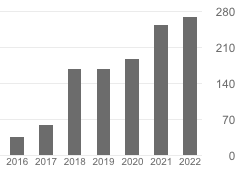
\includegraphics[height=30pt]{scholar-cit.png}

Names of students I supervise(d) are prepended with symbol \student{}.


\subsectionTitle{Rigorously Peer Reviewed Conferences}
\begin{pubs}

%%%%%%%%%%%%%%%%%%%%%%%%%%%%%%%%%%%%%%%%%%%%%%%%%%%%%%%%%%
%{\nemph{2025}}&\nemph{\rule{0.5\linewidth}{0.5pt}}\\[1em]

\confentry
	{78}
	{Prakhar Ganesh, \student{Cuong Tran}, Reza Shokri, {\bf Ferdinando Fioretto}}
	{The Data Minimization Principle in Machine Learning}
	{\procFAccT, 2025}
	{https://arxiv.org/abs/2405.19471}
	{26.8\%} % 812 submissions

\confentryAwd
	{77}
	{\student{Vincenzo Di Vito}, Mostafa Mohammadian, Kyri Baker, {\bf Ferdinando Fioretto}}
	{Learning To Solve Differential Equation Constrained Optimization Problems}
	{\procICLR, 2025}
	{https://arxiv.org/abs/2410.01786}
	{32.02\%} % 3,682 of 11,500 
	{[Spotlight]}{(5.1\% of the accepted papers / 0.01\% of all submitted papers.)}

\confentryAwd
	{76}
	{\student{Jacob K.~Christopher}, \student{Michael Cardei}, Brian R Bartoldson, Bhavya Kailkhura, {\bf Ferdinando Fioretto}}
	{Speculative Diffusion Decoding: Accelerating Language Generation through Diffusion}
	{\procNAACL, 2025}
	{https://arxiv.org/abs/2408.05636}
	{26\%}
	{[oral]}{(22\% of the accepted papers / 0.9\% of all submitted papers.)}

\confentry
	{75}
	{{\bf Ferdinando Fioretto}, Diptangshu Sen, Juba Ziani}
	{Differentially Private Data Release on Graphs: Inefficiencies and Unfairness}
	{\procAISTATS, 2025}
	{https://arxiv.org/abs/2408.05246}
	{31.3\%} %583/1861  

\confentryAwd
	{74}
	{\student{Joonhyuk Ko}, Juba Ziani, \student{Saswat Das}, Matt Williams, {\bf Ferdinando Fioretto}}
	{Fairness Issues and Mitigations in (Differentially Private) Socio-demographic Data Processes}
	{\procAAAI, 2025}
	{https://arxiv.org/abs/2408.08471}
	{19\%} % 89/469 (23)
	{[Oral]}{(5\% of the accepted papers.)}

\confentry
	{73}
	{FairDP: Certified Fairness with Differential Privacy}
	{Khang Tran, {\bf Ferdinando Fioretto}, Issa Khalil, My T.~Thai, NhatHai Phan}
	{In \venue{IEEE Secure and Trustworthy Machine Learning Conference (SaTML 2025)}, 2025}
	{https://arxiv.org/abs/2305.16474}
	{29.4\%}% 53/180

%%%%%%%%%%%%%%%%%%%%%%%%%%%%%%%%%%%%%%%%%%%%%%%%%%%%%%%%%%
%{\nemph{2024}}&\nemph{\rule{0.5\linewidth}{0.5pt}}\\[1em]

\confentry
	{72}
	{\student{Jacob K.~Christopher}, Stephen Baek, {\bf Ferdinando Fioretto}}
  	{Constrained Synthesis with Projected Diffusion Models}
  	{\procNeurIPS, 2024}
	{https://arxiv.org/abs/2402.03559}
	{25.8\%}
	% Also appeared in the AI+ORMS 2025 Bridge program and several other workshops.

\confentryAwd
	{71}
	{\student{Jacob K.~Christopher}, Stephen Baek, {\bf Ferdinando Fioretto}}
  	{Physics-Aware Generative Diffusion Models for Micro-structure Material Design}
  	{\venue{AI 4 Material science, at NeurIPS}, 2024}
	{https://arxiv.org/abs/2402.03559}
	{39\%}
	{[Oral]}{(6\% of the accepted papers.)}

\confentry
	{70}
	{\student{Jacob K.~Christopher}, \student{Michael Cardei}, Brian R Bartoldson, Bhavya Kailkhura, {\bf Ferdinando Fioretto}}
	{Speculative Diffusion Decoding: Accelerating Language Generation through Diffusion}
	{\venue{Efficient Natural Language and Speech Processing (ENLSP), at NeurIPS}, 2024}
	{https://arxiv.org/abs/2408.0563605246}
	{29\%}

\confentry
	{69}
	{Ethan King, \student{James Kotary}, {\bf Ferdinando Fioretto}, Jan Drgona}
	{Metric Learning to Accelerate Convergence of Operator Splitting Methods for Differentiable Parametric Programming}
	{\venue{63rd IEEE Conference on Decision and Control (CDC)}, 2024}
	{https://arxiv.org/abs/2404.00882}
	{56.7\%}

\confentry
	{68}
	{\student{James Kotary}, \student{Vincenzo Di Vito}, \student{Jacob K.~Christopher}, Pascal Van Hentenryck, Ferdinando Fioretto}
	{Predict-Then-Optimize by Proxy: Learning Joint Models of Prediction and Optimization}
  	{\procECAI, 2024}
  	{https://arxiv.org/2311.13087}
  	{23.3\%} % 2,344 submissions and accepted 547

\confentry
	{67}
	{\student{Sree Harsha Nelaturu}, \student{Nishaanth Kanna Ravichandran}, \student{Cuong Tran}, Sara Hooker, and {\bf Ferdinando Fioretto}}
	{On The Fairness Impacts of Hardware Selection in Machine Learning}	
	{\procICML, 2024}
	{https://arxiv.org/abs/2312.03886}
	{27.5\%}

\confentry
	{66}
	{\student{Saswat Das}, Marco Romanelli, {\bf Ferdinando Fioretto}}
	{Disparate Impact on Group Accuracy of Linearization for Private Inference}
	{\procICML, 2024}
	{https://arxiv.org/abs/2402.03629}
	{27.5\%}

\confentry
	{65}
	{\student{My H.~Dinh}, \student{James Kotary}, {\bf Ferdinando Fioretto}}
	{End-to-End Learning for Fair Multiobjective Optimization Under Uncertainty}
	{\procUAI, 2024}
	{https://arxiv.org/abs/2402.07772}
	{27.0\%}

\confentry
	{64}%{ArXiv}
	{\student{Cuong Tran}, Keyu Zhu, Pascal Van Hentenryck, {\bf Ferdinando Fioretto}}
	{Fairness Increases Adversarial Vulnerability}
	{\procIJCAI, 2024}
	{https://arxiv.org/abs/2211.11835}
	{13.9\%}

\confentry
	{63}
	{\student{My H.~Dinh}, \student{James Kotary}, {\bf Ferdinando Fioretto}}
	{Learning Fair Ranking Policies via Differentiable Optimization of Ordered Weighted Averages}
	{\procFAccT, 2024}
	{https://arxiv.org/abs/2402.05252}
	{24.3\%}

\confentry
	{62}
	{{\bf Ferdinando Fioretto}, Keyu Zhu, Pascal Van Hentenryck, \student{Saswat Das}, Christine Task}
  	{Finding $\epsilon$ and $\delta$ of Traditional Disclosure Control Systems}
	{\procAAAI, 2024}
	{https://arxiv.org/abs/2301.12204}
	{23.75\%}

\confentry
	{61}
	{\student{My H.~Dinh}, \student{James Kotary}, {\bf Ferdinando Fioretto}}
	{Differentiable Approximations of Fair OWA Optimization}
	{\venue{Workshop on Differentiable Almost Everything, at ICML}, 2024}
	{https://arxiv.org/abs/2402.07772}
	{27.0\%}

\confentry
	{60}
	{{\bf Ferdinando Fioretto}}
	{The Data Minimization Principle in Machine Learning}
	{\venue{Workshop on Generative AI and Law, at ICML}, 2024}
	{https://arxiv.org/abs/2405.19471}
	{~30.0\%}

%%%%%%%%%%%%%%%%%%%%%%%%%%%%%%%%%%%%%%%%%%%%%%%%%%%%%%%%%%
%{\nemph{2023}}&\nemph{\rule{0.5\linewidth}{0.5pt}}\\[1em]

\confentry
	{60}
	{\student{Cuong Tran} and {\bf Ferdinando Fioretto}}
	{Data Minimization at Inference Time}
	{\procNeurIPS, 2023}
	{https://arxiv.org/abs/2305.17593}
	{23.0\%}

\confentry
	{59}
 	{Vladimir Dvorkin and {\bf Ferdinando Fioretto}}
  	{Price-Aware Deep Learning for Electricity Markets}
  	{\venue{Tackling Climate Change with Machine Learning, at NeurIPS}, 2023}
  	{https://arXiv.org/abs/2308.01436}
  	{35.0\%}

\confentry 
	{58} %{IJCAI}
	{\student{James Kotary}, \student{My H.~Dinh}, {\bf Ferdinando Fioretto}}
	{Folded Optimization for End-to-End Model-Based Learning}
	{\procIJCAI, 2023}
	{https://arxiv.org/abs/2301.12047}
	{15.0\%}

\confentry
    {57} %{IJCAI}
	{\student{James Kotary}, \student{Vincenzo Di Vito}, {\bf Ferdinando Fioretto}, Pascal Van Hentenryck}
	{SF-PATE: Scalable, Fair, and Private Aggregation of Teacher Ensembles}
    {\procIJCAI, 2023}
	{https://arxiv.org/abs/2204.05157}
    {15.0\%}

\confentry
    {56} %{IJCAI}
	{\student{James Kotary}, \student{Vincenzo Di Vito}, {\bf Ferdinando Fioretto}}
	{End-to-End Combinatorial Ensemble Learning}
    {\procIJCAI, 2023}
	{http://arxiv.org/abs/2211.00251}
    {15.0\%}

\confentry
    {55} %{IJCAI}
	{\student{Cuong Tran}, {\bf Ferdinando Fioretto}}
	{On the Fairness Impacts of Private Ensembles Models}
    {\procIJCAI, 2023}
	{http://arxiv.org/abs/2109.08630}
    {15.0\%}

\confentry
	{54} %{PES}
	{Terrence W.K. Mak, {\bf Ferdinando Fioretto}, Pascal Van Hentenryck}
	{Load Encoding for Learning AC-OPF}
	{Proceedings of the \venue{IEEE PES General Meeting (PES)}, 2023}
	{https://arxiv.org/abs/2101.03973}
	{N/A}

\confentry
	{53}
	{\student{My H.~Dinh}, {\bf Ferdinando Fioretto}, Mostafa Mohammadian, and Kyri Baker}
	{An Analysis of the Reliability of AC Optimal Power Flow Deep Learning Proxies}
	{\venue{IEEE PES Innovative Smart Grid Technologies}, 2023}
	{https://arxiv.org/abs/2111.11168}
	{unknown}

\confentry
    {52} %{AAMAS}
	{\student{James Kotary}, \student{Vincenzo Di Vito}, {\bf Ferdinando Fioretto}}
	{End-to-End Optimization and Learning for Multiagent Ensembles}
    {\procAAMAS, 2023}
	{http://arxiv.org/abs/2211.00251}
    {40.0\%}

%%%%%%%%%%%%%%%%%%%%%%%%%%%%%%%%%%%%%%%%%%%%%%%%%%%%%%%%%%
%{\nemph{2022}}&\nemph{\rule{0.5\linewidth}{0.5pt}}\\[1em]

\confentryAwd
	{51} %{NeurIPS}
	{\student{Cuong Tran}, {\bf Ferdinando Fioretto}, Jung-Eun Kim, \student{Rakshit Naidu}}
	{Pruning has a disparate impact on model accuracy}
	{\procNeurIPS, 2022}
	{http://arxiv.org/abs/2205.13574}
	{25.6\%}
	{[Spotlight]}
	{($\sim$3\% of all paper submissions (10,411, in 2022).)}

	\confentry
	{50} %{IJCAI}
	{Keyu Zhu, {\bf Ferdinando Fioretto}, Pascal Van Hentenryck}
	{Post-processing of Differentially Private Data: A Fairness Perspective}
	{\procIJCAI, 2022}
	{http://arxiv.org/abs/2202.09425}	
	{15.0\%}

	\confentry
	{49} %{IJCAI}
	{{\bf Ferdinando Fioretto}, \student{Cuong Tran}, Keyu Zhu, Pascal Van Hentenryck}
	{Differential Privacy and Fairness in Decisions and Learning Tasks: A Survey}
	{\procIJCAI, 2022}
	{http://arxiv.org/abs/2202.08187}	
	{18.0\% (survey track)}

	\confentryAwd
	{48} %{IJCAI}
	{{\bf Ferdinando Fioretto}}
	{Integrating Machine Learning and Optimization to Boost Decision Making}
	{\procIJCAI, 2022}
	{https://web.ecs.syr.edu/~ffiorett/files/papers/Fioretto-IJCAI22-EC.pdf}	
	{Invited}
	{[Early Career Spotlight]}
	{(Accompanying paper.)}

	\confentry
	{47} %{WWW}
	{\student{James Kotary}, {\bf Ferdinando Fioretto}, Pascal Van Hentenryck, Ziwei Zhu}
	{End-to-end Learning for Fair Ranking Systems}
	{\procWWW, 2022}
	{http://arxiv.org/abs/2111.10723}	
	{17.0\%}
	
	\confentry
	{46} %{AAAI} 
	{\student{James Kotary}, {\bf Ferdinando Fioretto}, Pascal Van Hentenryck}
	{Fast Approximations for Job Shop Scheduling: A Lagrangian Dual Deep Learning Method}
	{\procAAAI, 2022}
	{http://arxiv.org/abs/2110.06365}
	{15.0\%}

	\confentry
	{45} %{PMAPS}
	{Lesia Mitridati, Emma Romei, Gabriela Hug, {\bf Ferdinando Fioretto}}
	{Differentially-Private Heat and Electricity Markets Coordination}
	{\procPMAPS, 2022}
	{https://arxiv.org/abs/2201.10634}
	{N/A}

	\confentry
	{44} %{PMAPS}
	{Mostafa Mohammadian, Kyri Baker, \student{My H.~Dinh}, {\bf Ferdinando Fioretto}}
	{Learning Solutions for Intertemporal Power Systems Optimization with Recurrent Neural Networks}
	{\procPMAPS, 2022}
	{https://ieeexplore.ieee.org/document/9810638}
	{N/A}

%%%%%%%%%%%%%%%%%%%%%%%%%%%%%%%%%%%%%%%%%%%%%%%%%%%%%%%%%%
%{\nemph{2021}}&\nemph{\rule{0.5\linewidth}{0.5pt}}\\[1em]

	\confentry 
	{43} %{NeurIPS}
	{\student{Cuong Tran}, \student{My H.~Dinh}, {\bf Ferdinando Fioretto}}
	{Differentially Private Deep Learning under the Fairness Lens}
	{\procNeurIPS, 2021}
	{https://arxiv.org/pdf/2106.02674.pdf}
	{26.0\%} % 9122

	\confentry 
	{42} %{NeurIPS}
	{\student{James Kotary}, {\bf Ferdinando Fioretto}, Pascal Van Hentenryck}
	{Learning Hard Optimization Problems: A Data Generation Perspective}
	{\procNeurIPS, 2021}
	{https://arxiv.org/pdf/2106.02674.pdf}
	{26.0\%} % 9122

	\confentryAwd 
	{41} %{IJCAI}
	{\student{Cuong Tran}, {\bf Ferdinando Fioretto}, Pascal Van Hentenryck, \student{Zhiyan Yao}}
	{Decision Making with Differential Privacy under the Fairness Lens}
	{\procIJCAI, 560--566, 2021}
	{https://www.ijcai.org/proceedings/2021/78}
	{13.9\%} %4,204/587
	{[Winner of the 2022 Caspar Bowden PET Award]}
	{(Selected among all papers about Privacy Enhancing Technologies published in international conferences between 2020--2022.)}

	\confentry 
	{40} %{IJCAI}
	{\student{James Kotary}, {\bf Ferdinando Fioretto}, Pascal Van Hentenryck, Bryan Wilder}
	{End-to-End Constrained Optimization Learning: A Survey}
	{\procIJCAI, 4475--4482, 2021}
	{https://www.ijcai.org/proceedings/2021/610}
	{30.1\%}

	\confentry 
	{39} %{AAAI}
	{Keyu Zhu, Pascal Van Hentenryck, {\bf Ferdinando Fioretto}}
	{Bias and Variance of Post-processing in Differential Privacy}
	{\procAAAI, 11177--11184, 2021}
	{https://ojs.aaai.org/index.php/AAAI/article/view/17333}
    {21.0\%} %  7,911/1,692

	\confentry 
	{38} %{AAAI}
	{\student{Cuong Tran}, {\bf Ferdinando Fioretto}, Pascal Van Hentenryck}
	{Differentially Private and Fair Deep Learning: A Lagrangian Dual Approach}
	{\procAAAI, 9932--9939, 2021}
	{https://ojs.aaai.org/index.php/AAAI/article/view/17193}
    {21.0\%} %  7,911/1,692

    \confentry
    {37} %{AAMAS}
    {\student{Anudit Nagar}, \student{Cuong Tran}, {\bf Ferdinando Fioretto}}
    {A Privacy-Preserving and Accountable Multi-agent Learning Framework}
    {\procAAMAS, 1605--1606, 2021}
    {https://dl.acm.org/doi/10.5555/3463952.3464174}
    {40.0\%}

	\confentry
	{36} %{CP}
	{\bf Ferdinando Fioretto}
	{Constrained-based Differential Privacy}
	{\procCP, 1868--8969, 2021}
	{https://drops.dagstuhl.de/opus/volltexte/2021/15293/}
	{Invited}
	
	\confentry 
	{35} %{PowerTech}
	{Vladimir~Dvorkin, {\bf Ferdinando Fioretto}, Pascal Van Hentenryck, Jalal~Kazempour, Pierre~Pinson}
	{Differentially Private Optimal Power Flow for Distribution Grids}
	{\venue{IEEE PowerTech}, 2021}
	{https://ieeexplore.ieee.org/document/9226144}
	{N/A} %4,204/587

%%%%%%%%%%%%%%%%%%%%%%%%%%%%%%%%%%%%%%%%%%%%%%%%%%%%%%%%%%
%{\nemph{2020}}&\nemph{\rule{0.5\linewidth}{0.5pt}}\\[1em]
	\confentry
		{34} %{ECML}
		{{\bf Ferdinando Fioretto}, Pascal Van Hentenryck, Terrence W.K. Mak, \student{Cuong Tran}, Federico Baldo, Michele Lombardi} 
		{A Lagrangian Dual Framework for Deep Neural Networks with Constraints}
		{\procECML, 18--135, 2020}
		{https://arxiv.org/abs/2001.09394}
		{19.0\%}

	\confentry
		{33} %{IJCAI}
		{{\bf Ferdinando Fioretto}, Lesia Mitridati, Pascal Van Hentenryck}
		{Differential Privacy Stackebelg Games}
		{\procIJCAI, 3480--3486, 2020}
		{https://www.ijcai.org/proceedings/2020/0481.pdf}
	    {12.6\%}

	\confentryAwd
		{32} %{IJCAI}
		{{\bf Ferdinando Fioretto}, Pascal Van Hentenryck}
		{OptStream: Releasing Time Series Privately}
		{\procIJCAI, 5135--5139, 2020}
	    {https://www.ijcai.org/proceedings/2020/722}
		{[Invited to the IJCAI journal track]}
		{(selected papers only.)}{}
	
	\confentry
		{31} %{PSCC}
		{Terrence W.K.~Mak, {\bf Ferdinando Fioretto}, Pascal Van Hentenryck}
		{Privacy-Preserving Obfuscation for Distributed Power Systems}
		{\procPSCC, 2020}
		{https://arxiv.org/abs/1910.04250}
	    {20.5\%} %  7,737/1591

	\confentry
		{30} %{AAAI}
		{{\bf Ferdinando Fioretto}, Terrence W.K.~Mak, Pascal Van Hentenryck}
		{Predicting AC Optimal Power Flows: Combining Deep Learning and Lagrangian Dual Methods}
	  	{\procAAAI, pages 630--637, 2020}
	  	{https://ojs.aaai.org//index.php/AAAI/article/view/5403}
	    {20.6\%} %  7,737/1591

	\confentry
		{29} %{PRIMA}
	    {Atena Tabakhi, William Yeoh, {\bf Ferdinando Fioretto}}
	    {The Smart Appliance Scheduling Problem: A Bayesian Optimization Approach}
	    {\procPRIMA, 100--115, 2020}
	    {https://link.springer.com/chapter/10.1007\%2F978-3-030-69322-0\_7}
	    {38.0\%} % 19/50

%%%%%%%%%%%%%%%%%%%%%%%%%%%%%%%%%%%%%%%%%%%%%%%%%%%%%%%%%%
%{\nemph{2019}}&\nemph{\rule{0.5\linewidth}{0.5pt}}\\[1em]
	\confentry
		{28} %{AAMAS}
		{{\bf Ferdinando Fioretto}, Pascal Van~Hentenryck}
		{Privacy-Preserving Federated Data Sharing}
	  	{\procAAMAS, pages 638--646, 2019}
	  	{https://dl.acm.org/doi/abs/10.5555/3306127.3331750}
		{24.0\%} % 189/781

	\confentry
		{27} %{IJCAI}
		{{\bf Ferdinando Fioretto}, Terrence W.K.~Mak, Pascal Van Hentenryck}
		{Privacy-Preserving Obfuscation of Critical Infrastructure Networks}
	  	{\procIJCAI, pages 1086--1092, 2019}
	  	{https://www.ijcai.org/proceedings/2019/0152.pdf}
	    {17.9\%} %  4,752/850

	\confentryAwd
		{26} %{CP}
		{{\bf Ferdinando Fioretto}, Pascal Van Hentenryck}
		%\href{https://web.ecs.syr.edu/~ffiorett/files/papers/cp19.pdf}
		{Differential Privacy of Hierarchical Census Data: An Optimization Approach} 
		{\procCP, pages 639--655, 2019}
		{https://link.springer.com/chapter/10.1007/978-3-030-30048-7\_37}
		{37.0\%}
		{[Invited to Constraint journal]}
		{(selected papers -- declined.)}

%%%%%%%%%%%%%%%%%%%%%%%%%%%%%%%%%%%%%%%%%%%%%%%%%%%%%%%%%%
%{\nemph{2018}}&\nemph{\rule{0.5\linewidth}{0.5pt}}\\[1em]
	\confentry 
		{25} %{PRIMA}
		{{\bf Ferdinando Fioretto}, Hong Xu, Sven Koenig, TK Satish Kumar}
	 	{Solving Multiagent Constraint Optimization Problems on the Constraint Composite Graph}
		{\procPRIMA, pages 106--122, 2018}
		{https://link.springer.com/chapter/10.1007/978-3-030-03098-8\_7}
	    {26.2\%} % 27/103

	\confentry
		{24} %{AAMAS}
	  	{{\bf Ferdinando Fioretto}, Chansoo Lee, Pascal Van Hentenryck}
	  	{Constrained-based Differential Privacy for Private Mobility} 
	  	{\procAAMAS, pages 1405--1413, 2018}
	  	{https://dl.acm.org/doi/abs/10.5555/3237383.3237910}
	    {25.2\%} % 151/597

	\confentry 
		{23} %{CP}
		{Khoi Hoang, {\bf Ferdinando Fioretto}, William Yeoh, Enrico Pontelli, Roie Zivan}
		{A Large Neighboring Search Schema for Multi-Agent Optimization}
		{\procCP, pages 688--706, 2018}
		{https://link.springer.com/chapter/10.1007/978-3-319-98334-9\_44}
	    {33.0\%} % 3/9 (in this track)

	\confentry 
		{22} %{CPAIOR}
		{{\bf Ferdinando Fioretto}, Pascal Van Hentenryck}
		{Constrained-based Differential Privacy: Releasing Optimal Power Flow Benchmarks Privately} 
		{\procCPAIOR, pages 215--231, 2018}
		{https://link.springer.com/chapter/10.1007/978-3-319-93031-2\_15}
	    {48.0\%}

	\confentry
		{21} %{ISIAM}
		{{\bf Ferdinando Fioretto}, Hong Xu, Sven Koenig, TK Satish Kumar}
		{Constraint Composite Graph-Based Lifted Message Passing for Distributed Constraint Optimization Problems}
		{\procISIAM, 2018}
		{https://speakerdeck.com/xuphys/constraint-composite-graph-based-lifted-message-passing-for-distributed-constraint-optimization-problems}
		{N/A}

%%%%%%%%%%%%%%%%%%%%%%%%%%%%%%%%%%%%%%%%%%%%%%%%%%%%%%%%%%
%{\nemph{2017}}&\nemph{\rule{0.5\linewidth}{0.5pt}}\\[1em]
	\confentry 
		{20} %{AAMAS}
		{{\bf Ferdinando Fioretto}, William Yeoh, Enrico Pontelli, Ye Ma, Satishkumar J.~Ranade}
		{A Distributed Constraint Optimization (DCOP) Approach to the Economic Dispatch with Demand Response}
		{\procAAMAS, pages  999--1007, 2017}
		{https://dl.acm.org/doi/10.5555/3091125.3091267}
		{24.9\%}%{\it 137/550 = 25\%}.

	\confentry 
		{19} %{AAMAS}
		{{\bf Ferdinando Fioretto},  William Yeoh, Enrico Pontelli}
		{A Multiagent System Approach to Scheduling Devices in Smart Homes}
		{\procAAMAS, pages 981--989, 2017} 
		{https://dl.acm.org/doi/10.5555/3091125.3091265}
		{24.9\%}%{\it 137/550 = 25\%}

	\confentry
		{18} %{AAMAS} 
		{Khoi Hoang, Ping Hou, {\bf Ferdinando Fioretto}, Makoto Yokoo, William Yeoh, Roie Zivan}
		{Infinite-Horizon Proactive Dynamic DCOPs}
		{\procAAMAS, pages 212--220, 2017}
		{https://dl.acm.org/doi/10.5555/3091125.3091160}
		{24.9\%}%{\it 137/550 = 25\%}.

	\confentry 
		{17} %{CP}
		{Atena M.~Tabakhi, Tiep Le, {\bf Ferdinando Fioretto}, William Yeoh}
		{Preference Elicitation for DCOPs}
		{\procCP, pages 278--296, 2017}
		{https://link.springer.com/chapter/10.1007/978-3-319-66158-2\_18}
		{43.0\%}%{\it 50+4/(137+17) = 25\%}.

%%%%%%%%%%%%%%%%%%%%%%%%%%%%%%%%%%%%%%%%%%%%%%%%%%%%%%%%%%
%{\nemph{$\leq$2016}}& \nemph{\rule{0.5\linewidth}{0.5pt}}\\[1em]
	\confentry 
		{16} %{AAMAS}
		{Khoi Hoang, {\bf Ferdinando Fioretto}, Ping Hou, Makoto Yokoo, William Yeoh, Roie Zivan}
		{Proactive Dynamic Distributed Constraint Optimization Problems} 
		{\procAAMAS, pages 597--605, 2016}
		{https://www.ifaamas.org/Proceedings/aamas2019/pdfs/p2411.pdf}
		{24.9\%}%{\it 137/550 = 25\%}.

	\confentry 
		{15} %{AAMAS}
		{Tiep Le, {\bf Ferdinando Fioretto}, William Yeoh, Enrico Pontelli, Tran Cao Son} 
		{ER-DCOPs: A Framework for Distributed Constraint Optimization Problems With Uncertainty} 
		{\procAAMAS,	pages 606--614, 2016}
		{https://dl.acm.org/doi/10.5555/2936924.2937014}
		{24.9\%}%{\it 137/550 = 25\%}.

	\confentry 
		{14} %{AAAI}
		{{\bf Ferdinando Fioretto}, William Yeoh, Enrico Pontelli}
		{Multi-Variable Agent Decompositions for DCOPs}
		{\procAAAI, pages 2480--2486, 2016}
		{https://dl.acm.org/doi/10.5555/3016100.3016246}
		{25.7\%}%{\it 549/2132 = 26\%}.

	\confentry
		{13} %{CP} 
		{{\bf Ferdinando Fioretto}, William Yeoh, Enrico Pontelli}
		{A Dynamic Programming-Based MCMC Framework for Solving DCOPs with GPUs}
		{\procCP, pages 813--831,	2016}
		{https://link.springer.com/chapter/10.1007/978-3-319-44953-1\_51}
		{35.0\%}%{\it 50+4/(137+17) = 34\%}.

%%%%%%%%%%%%%%%%%%%%%%%%%%%%%%%%%%%%%%%%%%%%%%%%%%%%%%%%%%
%%{\nemph{2015}}&\nemph{\rule{0.5\linewidth}{0.5pt}}\\[1em]
	\confentry
		{12} %{CP}
		{{\bf Ferdinando Fioretto}, Tiep Le, Enrico Pontelli, William Yeoh, Tran Cao Son}
		{Exploiting GPUs in Solving (Distributed) Constraint Optimization Problems with Dynamic Programming}
		{\procCP, pages 121--139, 2015}
		{https://dl.acm.org/doi/10.5555/3102787.3102797}
		{48.7\%}%{\it  39/80 = 49\%}.

	\confentry
		{11} %{AAMAS}
		{{\bf Ferdinando Fioretto}, Federico Campeotto, Agostino Dovier, Enrico Pontelli, William Yeoh}
		{Large Neighborhood Search with Quality Guarantees for Distributed Constraint Optimization Problems}
		{\procAAMAS, pages 1835--1836, 2015}
		{https://dl.acm.org/doi/10.5555/2772879.2773461}
		{46.0\%}

	\confentry
		{10} %{AAMAS}
		{{\bf Ferdinando Fioretto}, William Yeoh, Enrico Pontelli}
		{Multi-Variable Agents Decomposition for DCOPs to Exploit Multi-Level Parallelism}
		{\procAAMAS, pages 1823--1824, 2015}
		{https://dl.acm.org/doi/10.5555/2772879.2773455}
		{46.0\%}

	\confentry
		{9} %{AAMAS}
		{{\bf Ferdinando Fioretto}}
		{Exploiting the Structure of Distributed Constraint Optimization Problems} 
		{\procAAMAS, pages 2007--2008, 2015}
		{https://dl.acm.org/doi/10.5555/2772879.2773549}
		{N/A}

	\confentry
		{8} %{AAAI}
		{{\bf Ferdinando Fioretto}} 
		{Exploiting the Structure of Distributed Constraint Optimization Problems}
		{\procAAAI,  pages 4233--4234, 2015}
		{https://www.aaai.org/ocs/index.php/AAAI/AAAI15/paper/view/9293}
		{N/A}

%%%%%%%%%%%%%%%%%%%%%%%%%%%%%%%%%%%%%%%%%%%%%%%%%%%%%%%%%%
%%{\nemph{$\leq$2014}}&\nemph{\rule{0.5\linewidth}{0.5pt}}\\[1em]
	\confentry 
		{7} %{ECAI}
		{($\alpha$-$\beta$) 
		Federico Campeotto, Agostino Dovier, {\bf Ferdinando Fioretto}, Enrico Pontelli}
		{A GPU Implementation of Large Neighborhood Search for Solving Constraint Optimization Problems} 
		{\procECAI, pages 189--194, 2014}
		{https://dl.acm.org/doi/10.5555/3006652.3006685}
		{28.0\%}

	\confentry
		{6} %{CP}
		{{\bf Ferdinando Fioretto}, Tiep Le, William Yeoh, Enrico Pontelli, Tran Cao Son}
		{Improving DPOP with Branch Consistency for Solving Distributed Constraint Optimization Problems}
		{\procCP, pages 307--323, 2014}
		{https://link.springer.com/chapter/10.1007\%2F978-3-319-10428-7\_24}
		{49.8\%}
		
	\confentry
		{5} %{PADL}
		{($\alpha$-$\beta$) 
		Federico Campeotto, Alessandro Dal Pal\`{u}, Agostino Dovier, {\bf Ferdinando Fioretto}, Enrico Pontelli}
		{Exploring the Use of GPUs in Constraint Solving}
		{\procPADL, pages 152--167, 2014}
		{https://link.springer.com/chapter/10.1007\%2F978-3-319-04132-2\_11}
		{55.0\%}

	\confentry 
		{4} %{AAMAS}
		{{\bf Ferdinando Fioretto}, Federico Campeotto, Luca Da Rin Fioretto, William Yeoh, Enrico Pontelli} 
		{GD-Gibbs: A GPU-based Sampling Algorithm for Solving Distributed Constraint Optimization Problems} %(Extended Abstract)". 
		{\procAAMAS, pages 1339--1340, 2014}
		{https://dl.acm.org/doi/10.5555/2615731.2617462}
		{46.0\%}
	
	\confentryAwd
		{3} %{CMSB}
		{{\bf Ferdinando Fioretto}, Enrico Pontelli} 
		{Constraint Programming in Community-based Gene Regulatory Network Inference} 
		{\procCMSB, pages 135--149, 2013}
		{https://link.springer.com/chapter/10.1007\%2F978-3-642-40708-6\_11}
		{55.0\%}
		{[Best Student Paper Award]}{}

	\confentry 
		{2} %{CP}
		{($\alpha$-$\beta$) 
		Federico Campeotto, Alessandro Dal Pal\`{u}, Agostino Dovier, {\bf Ferdinando Fioretto}, Enrico Pontelli}
		{A Filtering Technique for Fragment Assembly-based Proteins Loop Modeling with Constraints} 
		{\procCP, pages 850--866, 2012}
		{https://link.springer.com/chapter/10.1007\%2F978-3-642-33558-7\_61}
		{36.0\%}

	\confentry
		{1} % {Neuroscience}
		{Michael R. Best, {\bf Ferdinando Fioretto}, Alessandro Dal Pal\`{u}, Enrico Pontelli, Tran Son, TuShun R. Powers, Elba E. Serrano}
		{The role of secondary and tertiary structure prediction in determining the function of novel genes found in Xenopus Leavis}
		{\venue{Neuroscience}, 2011, (518.20/ZZ45)}{}
		{N/A}
\end{pubs}


\subsectionTitle{Journals}
\begin{pubs}
\journalentry
	{14}
	{Jayanta Mandi, \student{James Kotary}, Senne Berden, Maxime Mulamba, Victor Bucarey, Tias Guns, {\bf Ferdinando Fioretto}} 
	{Decision-Focused Learning: Foundations, State of the Art, Benchmark and Future Opportunities}
	{\JAIR, (81), pages 1623--1701, 2024}
	{https://arxiv.org/abs/2307.13565}

	\journalentry
	{13}
	{Mostafa Mohammadian, Kyri Baker, \textbf{Ferdinando Fioretto}}
	{Gradient-Enhanced Physics-Informed Neural Networks for Power Systems Operational Support}
	{Electric Power Systems Research (223), pages 109551, 2023}
	{https://www.sciencedirect.com/science/article/abs/pii/S0378779623004406}

	\journalentry
	{12} %{JAIR}
	{Khoi D.~Hoang, \textbf{Ferdinando Fioretto}, Ping Hou, William Yeoh, Makoto Yokoo, Roie Zivan}
	{Proactive Dynamic Distributed Constraint Optimization Problems}
	{\JAIR, (73), pages 179-225, 2022}
	{https://www.jair.org/index.php/jair/article/view/13499}

	\journalentry
	{11} %{AIJ}
	{\textbf{Ferdinando Fioretto}, Pascal Van Hentenryck, Keyu Zhu}
	{Differential Privacy of Hierarchical Census Data: An Optimization Approach}
	{\AIJ, (296), pages 103475, 2021}
	{https://www.sciencedirect.com/science/article/pii/S0004370221000266}

	\journalentryAwd
	{10} %{IEEE-TPS}
	{Vladimir Dvorkin, {\bf Ferdinando Fioretto}, Pascal Van Hentenryck, Pierre Pinson, Jalal Kazempour}
	{Differentially Private Optimal Power Flow for Distribution Grids}
	{\TPS, 36(3), pages 2186--2196, 2021}
	{https://ieeexplore.ieee.org/document/9226144}
	{[Best IEEE TPS paper award]}
	{(Given to 8 out of all TPS papers published in 2019--2021.)}

	\journalentry
	{9} %{IEEE-TSG} 
	{{\bf Ferdinando Fioretto}, Terrence W.K.~Mak, Pascal Van Hentenryck}
	{Differential Privacy for Power Grid Obfuscation}
	{\TSG, 11(2), pages 1356--1366, 2020}
	{https://ieeexplore.ieee.org/document/8809257}

	\journalentryAwd
	{8}	%{IEEE-TPS}
	{Terrence W.K.~Mak, {\bf Ferdinando Fioretto}, \student{Lyndon Shi}, Pascal Van Hentenryck}
	{Privacy-Preserving Power System Obfuscation: A Bilevel Optimization Approach}
	{\TPS, 35(2), pages 1627--1637, 2020}
	{https://ieeexplore.ieee.org/document/8854890}
	{[Best IEEE TPS paper award]}
	{Given to 7 out of all TPS papers published in 2018--2020).}

	\journalentryAwd
	{7}	%{JAIR}
	{{\bf Ferdinando Fioretto}, Pascal Van Hentenryck}
	{OptStream: Releasing Time Series Privately}
	{\JAIR, (65) pages 423--456, 2019}
	{https://www.jair.org/index.php/jair/article/view/11583}
	{[Invited to IJCAI 2020 journal track]}
	{}

	\journalentryAwd
	{6}	%{IA}
	{{\bf Ferdinando Fioretto}, Agostino Dovier, Enrico Pontelli}
	{Distributed Multi-Agent Optimization for Smart Grids and Home Automation}
	{\venue{Intelligenza Artificiale (IA)},  12 (2), pages: 67--87, 2019}
	{https://content.iospress.com/articles/intelligenza-artificiale/ia180037}
	{[Best 2018 Thesis in Artificial Intelligence (AI*IA)]}
	{(Accompanying paper.)}

	\journalentry
	{5}	%{JAIR}
	{{\bf Ferdinando Fioretto}, Enrico Pontelli, William Yeoh}
	{Distributed Constraint Optimization Problems and Applications: A Survey}
	{\JAIR, 61, pages 623--698, 2018} 
	{https://arxiv.org/abs/1602.06347}

	\journalentry 
	{4}	%{AI Matters}
	{{\bf Ferdinando Fioretto}, William Yeoh}
	{AI Buzzwords Explained: Distributed Constraint Optimization Problems}
	{\venue{AI Matters}, 3 (4), pages 8--13, 2018}
	{https://sigai.acm.org/static/aimatters/3-4/AIMatters-3-4-04-Fioretto.pdf}

	\journalentry 
	{3}	%{Constraints}
	{{\bf Ferdinando Fioretto}, Enrico Pontelli, William Yeoh, Rina Dechter}
	{Accelerating Exact and Approximate Inference for (Distributed) Discrete Optimization with GPUs}
	{\venue{Constraints}, 23 (1), pages 1--43, 2018}
	{https://link.springer.com/article/10.1007/s10601-017-9274-1}

	\journalentry 
	{2}	%{TOMACS}
	{{\bf Ferdinando Fioretto}, Agostino Dovier, Enrico Pontelli}
	{Constrained Community-based Gene Regulatory Network Inference}
	{\venue{ACM Transactions on Modeling and Computer Simulation (TOMACS)}, 25 (2), pages 11:1--11:26, 2015}
	{https://dl.acm.org/doi/10.1145/2688909}

	\journalentry
	{1}	%{JAIR}
	{($\alpha$-$\beta$)\footnote{Author list is order alphabetically.} 
		Federico Campeotto, Alessandro Dal Pal\`{u}, Agostino Dovier,  {\bf Ferdinando Fioretto}, Enrico Pontelli}
	{A Constraint Solver for Flexible Protein Models}
	{\JAIR, 48, pages 953--1000, 2013}
	{https://www.jair.org/index.php/jair/article/view/10856}
\end{pubs}

\subsectionTitle{Book Chapters and Editorial Articles}
\begin{pubs}
\journalentry
	{6} %{AI Mag.}
	{{\bf Ferdinando Fioretto}, Pascal Van Hentenryck, and Juba Ziani}
	{Differential Privacy Overview and Fundamental Techniques}
	{{\bf DP Book}, forthcoming}
	{https://arxiv.org/abs/2411.04710}

\journalentry
	{5} %{AI Mag.}
	{{\bf Ferdinando Fioretto}, et al.} 
	{Reports of the Workshops Held at the 2022 AAAI Conference on Artificial Intelligence}
	{{\bf AI Magazine}, 2022}
	{https://interactiveaimag.org/updates/reports/reports-of-the-workshops-held-at-the-2022-aaai-conference-on-artificial-intelligence/}

\journalentry
	{4} %{AI Mag.}
	{{\bf Ferdinando Fioretto}, et al.} 
	{Reports of the Workshops Held at the 2021 AAAI Conference on Artificial Intelligence}
	{{\bf AI Magazine}, 2021}
	{https://interactiveaimag.org/updates/reports/reports-of-the-workshops-held-at-the-2021-aaai-conference-on-artificial-intelligence/}

\journalentry
	{3} %{AI Mag.}
	{{\bf Ferdinando Fioretto}, et al.} 
	{Reports of the Workshops Held at the 2020 International Association for the Advancement of Artificial Intelligence Conference on Web and Social Media}
	{{\bf AI Magazine},  41(4) 2020}
	{https://ojs.aaai.org/index.php/aimagazine/article/view/7486}

\journalentryAwd
	{2} %{LNCS}
	{\student{William Kluegel}, \student{Muhammad A.~Iqbal}, {\bf Ferdinando Fioretto}, William Yeoh, Enrico Pontelli}
	{A Realistic Dataset for the Smart Home Device Scheduling Problem for DCOPs}
	{\emph{Lecture Notes in Computer Science (LCNS)}, LNCS, volume 10643 pages 125--142, Springer, 2017}
	{https://link.springer.com/chapter/10.1007\%2F978-3-319-71679-4\_9}
	{Visionary Paper Award}
	{(AAMAS workshop series)}

\journalentry
	{1} %{LNBIP}
	{Moinul M.P.~Chowdhury, Russell Y.~Folk, {\bf Ferdinando Fioretto}, Christopher Kiekintveld, William Yeoh}
	{Investigation of Learning Strategies for the SPOT Broker in Power TAC}
	{\emph{AgentMediated Electronic Commerce: Designing Trading Strategies and Mechanisms for Electronic Markets}, volume 271 of Lecture Notes in Business Information Processing, 
	    pages 96–111, Springer, 2017}
    {https://link.springer.com/chapter/10.1007\%2F978-3-319-54229-4\_7}
\end{pubs}


\subsectionTitle{Peer Reviewed Workshops}
\begin{pubs}

\wsentryAwd
	{31} 
	{\student{Joonhyuk Ko}, Juba Ziani, \student{Saswat Das}, Matt Williams, {\bf Ferdinando Fioretto}}
	{Fairness Issues and Mitigations in (Differentially Private) Socio-demographic Data Processes}
	{\venue{AAAI Workshop on Privacy Preserving Artificial Intelligence  (PPAI)--at AAAI}, 2025}
	{https://arxiv.org/abs/2408.08471}
	{[Oral]}%{(11\% of the submitted papers.)}
	% Also appeared in the AI+ORMS 2025 Bridge program as an oral!

\wsentryAwd
	{30}
	{Low-rank finetuning for LLMs: A fairness perspective}
	{\student{Saswat Das}, Marco Romanelli, \student{Cuong Tran}, \student{Zarreen Reza}, Bhavya Kailkhura,  {\bf Ferdinando Fioretto}}
	{{\venue AAAI CoLoRAI Workshop}, 2025}
	{https://arxiv.org/abs/2405.18572}
	{[Best paper award]}


\wsentryAwd
	{29} 
	{\student{Jinhao Liang}, \student{Jacob Christopher}, Sven Koenig, {\bf Ferdinando Fioretto}}
	{Multi-Agent Path Finding in Continuous Spaces with Projected Diffusion Models}
	{\venue{Combining AI and OR/MS for Better Trustworthy Decision Making, at AAAI}, 2025}
	{}
	{[Oral]}
	% Also appeared in the AI+ORMS 2025 Bridge program as an oral!

\wsentry
	{28}
	{\student{Vincenzo Di Vito}, Mostafa Mohammadian, Kyri Baker, {\bf Ferdinando Fioretto}}
	{OPF-Net: Real-Time Stability Constrained AC Optimal Power Flow}
	{\venue{AAAI Bridge on Explainable AI, Energy and Critical Infrastructure Systems}, 2025}
	{https://arxiv.org/abs/2410.19157}

\wsentry
	{27}
	{\student{Jacob K.~Christopher}, Stephen Baek, {\bf Ferdinando Fioretto}}
	{Physics-Aware Diffusion Models for Micro-structure Material Design}
	{\venue{ELLIS ML for Molecules and Materials in the Era of LLMs Workshop, 2024}}
	{}

\wsentry
	{26}
	{\student{Jacob K.~Christopher}, Michael Cardei, Brian R Bartoldson, Bhavya Kailkhura, {\bf Ferdinando Fioretto}}
	{Speculative Diffusion Decoding: Accelerating Language Generation through Diffusion}
	{\venue{Efficient Natural Language and Speech Processing (ENLSP) workshop -- at NeurIPS}, 2024}
	{https://arxiv.org/abs/2408.0563605246}

\wsentry
 	{25}
	{\student{Jacob K.~Christopher}, Stephen Baek, {\bf Ferdinando Fioretto}}
  	{Constrained Synthesis with Projected Diffusion Models}
  	{\venue{Machine Learning and the Physical Sciences Workshop -- at NeurIPS}, 2024}
	{https://arxiv.org/abs/2402.03559}

\wsentry
	{24}
	{Prakhar Ganesh, \student{Cuong Tran}, Reza Shokri, {\bf Ferdinando Fioretto}}
	{The Data Minimization Principle in Machine Learning}
	{\venue{Workshop on Regulatory ML -- at NeurIPS}, 2024}
	{https://arxiv.org/abs/2405.19471}

\wsentry
	{23}
	{\student{My H.~Dinh}, \student{James Kotary}, {\bf Ferdinando Fioretto}}
	{Differentiable Approximations of Fair OWA Optimization}
	{\venue{Workshop on Differentiable Almost Everything -- at ICML}, 2024}
	{https://arxiv.org/abs/2402.07772}

\wsentry
	{22}
	{{\bf Ferdinando Fioretto}}
	{The Data Minimization Principle in Machine Learning}
	{\venue{Workshop on Generative AI and Law -- at ICML}, 2024}
	{https://arxiv.org/abs/2405.19471}

\wsentry 
	{21}%{ArXiv}
	{Vladimir Dvorkin, {\bf Ferdinando Fioretto}, Pascal Van Hentenryck, Pierre Pinson, Jalal Kazempour}
	{Privacy-Preserving Convex Optimization: When Differential Privacy Meets Stochastic Programming}
	{\venue{Workshop on Climate Change AI -- at NeurIPS}, 2023}
	{http://arxiv.org/abs/2209.14152}


	\wsentryAwd
	{20} %{PPAI}
	{\student{Cuong Tran}, \student{My H.~Dinh}, {\bf Ferdinando Fioretto}}
	{A Fairness Analysis on Private Aggregation of Teacher Ensembles}
	{\venue{AAAI Workshop on Privacy Preserving Artificial Intelligence 
		(PPAI)--at AAAI}, 2022}
	{http://arxiv.org/abs/2109.08630}
	{Spotlight Paper}
	
	\wsentry
	{19} %{TPDP}
	{\student{Cuong Tran}, {\bf Ferdinando Fioretto}}
	{Decision Making with Differential Privacy under the Fairness Lens}
	{\venue{Theory and Practice of Differential Privacy (TPDP) -- at ICML}, 2021}
	{https://tpdp.journalprivacyconfidentiality.org/2021/}
 	
	\wsentry
	{18} %{OptLMAS}
	{\student{Anudit Nagar}, \student{Cuong Tran}, {\bf Ferdinando Fioretto}}
	{A Privacy-Preserving and Accountable Multi-agent Learning Framework}
	{\venue{International Workshop on Learning and Optimization 
 		   in Multi-Agent Systems (OPTLearnMAS)--at AAMAS}, 2021}
	{https://optlearnmas21.github.io/}

	\wsentry
	{17} %{PPAI}
	{\student{Cuong Tran}, {\bf Ferdinando Fioretto}, Pascal Van~Hentenryck}
	{Differentially Private and Fair Deep Learning: A Lagrangian Dual Approach}
	{\venue{AAAI Workshop on Privacy Preserving Artificial Intelligence 
		(PPAI)--at AAAI}, 2021}
	{https://arxiv.org/abs/2009.12562}

\wsentry 
	{16} %{INFORMS}
	{{\bf Ferdinando Fioretto}, \student{Cuong Tran}, Pascal Van Hentenryck}
	{Lagrangian Duality for Constrained Deep Learning}
	{\venue{INFORMS}, 2020}
	{http://meetings2.informs.org/wordpress/annual2020/}

\wsentry 
	{15} %{INFORMS}
	{Lesia Mitridati, {\bf Ferdinando Fioretto}, Pascal Van Hentenryck}
	{Differential Privacy For Stackelberg Games: An Application To Gas And Electricity Markets}
	{\venue{INFORMS}, 2020}
	{http://meetings2.informs.org/wordpress/annual2020/}


\wsentry 
	{14} %{OptMAS}
	{Khoi Hoang, {\bf Ferdinando Fioretto}, William Yeoh, Enrico Pontelli, Roie Zivan}
	{A Large Neighboring Search Schema for Multi-Agent Optimization} 
	{\venue{International Workshop on Optimization 
 		   in Multi-Agent Systems (OPTMAS)--at AAMAS}, 2019}
	{https://www2.isye.gatech.edu/~fferdinando3/cfp/OPTMAS19/}

\wsentry
	{13} %{OptMAS}
	{{\bf Ferdinando Fioretto}, Hong Xu, Sven Koenig, TK Satish Kumar}
	{Solving Multiagent Constraint Optimization Problems on the Constraint Composite Graph} 
	{\venue{International Workshop on Optimisation in Multi-Agent Systems 
	(OptMAS)--at AAMAS}, 2018}
	{~}

\wsentry
	{12} %{OptMAS}	
	{William Kluegel, Muhammad Aamir Iqbal, {\bf Ferdinando Fioretto}, William Yeoh, Enrico Pontelli}
	{A Realistic Dataset for the Smart Home Device Scheduling Problem for DCOPs}
	{\venue{International Workshop on Optimisation in Multi-Agent Systems (OPTMAS)--at AAMAS}, 
	2017}
	{~}	

\wsentry
	{11} %{AISGSB}
	{{\bf Ferdinando Fioretto},  William Yeoh, Enrico Pontelli}
	{A Multiagent System Approach to Scheduling Devices in Smart Homes}
	{\venue{Workshop on AI for Smart Grids and Smart Buildings (AISGSB)--at AAAI}, 2017}
	{~}

	\wsentry
	{10} %{MPREF} 
	{Atena M.~Tabakhi, {\bf Ferdinando Fioretto}, William Yeoh}
	{A Preliminary Study on Preference Elicitation in DCOPs for Scheduling Devices in Smart Buildings}
	{\venue{10th Workshop on Advances in Preference Handling (MPREF)--at IJCAI}, 2016}
	{~}

\wsentry 
	{9} %{TADA}
	{Porag Chowdhury, Russell Y. Folk, {\bf Ferdinando Fioretto}, Christopher Kiekintveld, William Yeoh}
	{Investigation of Learning Strategies for the SPOT Broker in Power TAC}
  	{\venue{International Workshop on Agent Mediated Electronic Commerce and Trading Agents Design and Analysis
	(AMEC/TADA)--at AAMAS}, 2016}
	{~}

\wsentry 
	{8} %{AISGSB}
	{Khoi Hoang, {\bf Ferdinando Fioretto}, Ping Hou, Makoto Yokoo, William Yeoh, Roie Zivan}
	{Proactive Dynamic DCOPs} 
	{\venue{Workshop on AI for Smart Grids and Smart Buildings (AISGSB)--at AAAI}, 2016}
	{~}	

\wsentry
	{7} %{OptMAS} 
	{{\bf Ferdinando Fioretto}, Federico Campeotto, Agostino Dovier, Enrico Pontelli, William Yeoh}
	{Large Neighborhood Search with Quality Guarantees for Distributed Constraint Optimization Problems} 
	{In \venue{International Workshop on Optimization in Multi-Agent Systems (OptMAS)-- at AAMAS}, 2015}
	{~}

\wsentry 
	{6} %{OptMAS}
	{{\bf Ferdinando Fioretto}, Tiep Le, William Yeoh, Enrico Pontelli, Tran Cao Son}
	{Improving DPOP with Branch Consistency for Solving Distributed Constraint Optimization Problems}
	{In \venue{International Workshop on Optimization in Multi-Agent Systems (OptMAS)-- at AAMAS}, 2015}
	{~}

\wsentry 
	{5} %{WCB}
	{($\alpha$-$\beta$) 
	Federico Campeotto, Alessandro Dal Pal\`{u}, Agostino Dovier, {\bf Ferdinando Fioretto}, Enrico Pontelli} 
  	{Experimenting with FIASCO for protein structure prediction}
	{\venue{Workshop on Constraint Based Methods for Bioinformatics (WCB)--at CP}, 2014}
	{~}

\wsentry 
	{4} %{ParSeachOpt}
	{($\alpha$-$\beta$) Federico Campeotto, Alessandro Dal Pal\`{u}, Agostino Dovier, {\bf Ferdinando Fioretto}, Enrico Pontelli}
	{Towards a complete constraint solver on GPU}
	{In \venue{Workshop on Parallel Methods for Search \& Optimization (ParSearchOpt)--at ECAI}, 2014}
	{~}

\wsentry 
	{3} %{WCB}
	{{\bf Ferdinando Fioretto}, Enrico Pontelli}
	{Community-based Gene Regulatory Network Inference via Constraint Programming}
	{\venue{Workshop on Constraint Based Methods for Bioinformatics (WCB)--at CP}, 2013}
	{~} 

\wsentry
	{2} %{WCB} 
	{($\alpha$-$\beta$) 
	Federico Campeotto, Alessandro Dal Pal\`{u}, Agostino Dovier, {\bf Ferdinando Fioretto}, Enrico Pontelli}
	{Protein Loop Modelling via Constraints and Fragment Assembly}
	{\venue{Workshop on Constraint Based Methods for Bioinformatics (WCB)--at CP}, 2012}
	{~} 

\wsentry 
	{1} %{WCB}
	{($\alpha$-$\beta$) 
	Michael R. Best, Kabi Bhattarai, Federico Campeotto, Alessandro Dal Pal\`{u}, Hung Dang, Agostino Dovier, {\bf Ferdinando Fioretto}, Federico Fogolari, Tiep Le, Enrico Pontelli}
		{Introducing FIASCO: Fragment-based Interactive Assembly for protein Structure prediction with COnstraints}
 	 {\venue{Workshop on Constraint Based Methods for  Bioinformatics (WCB)--at CP}, 2011}
  	{~}
\end{pubs}


\subsectionTitle{Pre-prints and In-press}
\begin{pubs}
\wsentry
	{11}
	{\student{Michael Cardei}, \student{Jacob K Christopher}, Thomas Hartvigsen, Brian R. Bartoldson, Bhavya Kailkhura, and Ferdinando Fioretto}
	{Constrained Language Generation with Discrete Diffusion Models}
	{\venue{TBD}, 2025}
	{https://arxiv.org/abs/2503.09790}

\wsentry
	{10}
	{Shuyi Chen, Ferdinando Fioretto, Feng Qiu, Shixiang Zhu}
	{Global-Decision-Focused Neural ODEs for Proactive Grid Resilience Management}
	{\venue{IEEE Transactions on Smart Grids}  (under review), 2025}
	{https://arxiv.org/abs/2502.18321}
	
\wsentry
	{9}
	{\student{Jinhao Liang}, \student{Jacob K Christopher}, Sven Koenig, {\bf Ferdinando Fioretto}}
	{Simultaneous Multi-Robot Motion Planning with Projected Diffusion Models}
	{\venue{ICML} (under review), 2025}
	{https://arxiv.org/}

\wsentry
	{8}
	{\student{Stefano Zampini}, \student{Jacob K Christopher}, Luca Oneto, Davide Anguita, {\bf Ferdinando Fioretto}}
	{Training-Free Constrained Generation With Stable Diffusion Models}
	{\venue{ICML} (under review), 2025}
	{https://arxiv.org/}

\wsentry
	{7}
	{Prince Zizhuang Wang, \student{Jinhao Liang}, Shuyi Chen, {\bf Ferdinando Fioretto}, Shixiang Zhu}
	{Gen-DFL: Decision-Focused Generative Learning for Robust Decision Making}
	{\venue{ICML} (under review), 2025}
	{https://arxiv.org/}


\wsentry
	{6}
	{\student{Jinhao Liang}, \student{Jacob K.~Christopher}, Sven Koenig, Ferdinando Fioretto} 
	{Multi-Agent Path Finding in Continuous Spaces with Projected Diffusion Models}
	{\venue{CoRR abs}/2412.17993, 2025}
	{https://arxiv.org/abs/2412.17993}

\wsentry
	{5}
	{\student{Vincenzo Di Vito}, Mostafa Mohammadian, Kyri Baker, {\bf Ferdinando Fioretto}}
	{OPF-Net: Real-Time Stability Constrained AC Optimal Power Flow}
	{\venue{IEEE Transactions on Power Systems} (revision), 2025}
	{https://arxiv.org/abs/2410.19157}

\wsentry
	{4}
	{\student{My H.~Dinh}, \student{James Kotary}, Lauryn P.~Gouldin, William Yeoh, {\bf Ferdinando Fioretto}}
	{End-to-End Optimization and Learning of Fair Court Schedules}
	{\venue{FAccT} (under review), 2025}
	{https://arxiv.org/abs/2410.17415}

\wsentry
	{3}
	{\student{Saswat Das},  Marco Romanelli, \student{Cuong Tran}, \student{Zarreen Reza}, 
	Bhavya Kailkhura, {\bf Ferdinando Fioretto}}
	{Low-rank finetuning for LLMs: A fairness perspective}
	{\venue{FAccT} (under review), 2025}
	{https://arxiv.org/abs/2405.18572}


\wsentry
	{2}
	{\student{James Kotary}, {\bf Ferdinando Fioretto}}
	{Learning Constrained Optimization with Deep Augmented Lagrangian Methods}
	{\venue{CoRR abs}/2403.03454, 2024}
	{https://arxiv.org/abs/2403.03454}

\wsentry
	{1}
	{\student{James Kotary}, \student{Jacob K.~Christopher}, \student{My H Dinh},
	and {\bf Ferdinando Fioretto}}
	{Analyzing and Enhancing the Backward-Pass Convergence of Unrolled Optimization}	
	{\venue{INFORMS journal of computing} (under review), 2024}
	{https://arxiv.org/abs/2301.12047}

\end{pubs}


%--------------------------------------------------------------------
%	Conference: Archieved Papers
%--------------------------------------------------------------------
\subsectionTitle{Archived and Extended Versions of Published Papers}
\begin{pubs}

\wsentry 
	{12}%{ArXiv}
	{\student{My H.~Dinh}, {\bf Ferdinando Fioretto}}
	{Context-Aware Differential Privacy for Language Modeling}
	{\venue{CoRR abs}/2301.12288, 2023}
	{https://arxiv.org/abs/2301.12288}

\wsentry 
	{11}%{ArXiv}
	{Sawinder Kaur, {\bf Ferdinando Fioretto}, Asif Salekin}
	{Deadwooding: Robust Global Pruning for Deep Neural Networks} 
	{\venue{CoRR abs}/2202.05226, 2022}
	{http://arxiv.org/abs/2202.05226}

\wsentry 
	{10}%{ArXiv}
	{\student{My H.~Dinh}, {\bf Ferdinando Fioretto}, Mostafa Mohammadian, Kyri Baker}
	{Towards Understanding the Unreasonable Effectiveness of Learning AC-OPF Solutions}
	{\venue{CoRR abs}/2111.11168, 2021}
	{http://arxiv.org/abs/2111.11168}

\wsentry % (NeruIPS-21)
	{9}%{ArXiv}
	{\student{Cuong Tran}, \student{My H.~Dinh}, {\bf Ferdinando Fioretto}}
	{Differentially Private Deep Learning under the Fairness Lens}
	{\venue{CoRR abs}/2106.02674, 2021 ({\bf extended NeurIPS-21 version})}
	{http://arxiv.org/abs/2106.02674}

\wsentry 
	{8}%{ArXiv}
	{\student{Anudit Nagar}, \student{Cuong Tran}, {\bf Ferdinando Fioretto}}
	{A Privacy-Preserving and Trustable Multi-agent Learning Framework}
	{\venue{CoRR abs}/2106.01242, 2021. ({\bf extended AAMAS-21 version})}
	{https://arxiv.org/abs/2106.01242}

\wsentry % (IJCAI-21 )
	{7}%{ArXiv}
	{\student{James Kotary}, {\bf Ferdinando Fioretto}, Pascal Van Hentenryck, Bryan Wilder}
	{End-to-End Constrained Optimization Learning: A Survey}
	{\venue{CoRR abs}/2103.16378, 2021. ({\bf extended IJCAI-21 version})}
	{https://arxiv.org/abs/2103.16378}

\wsentry 
	{6}%{ArXiv}
	{Terrence W.K. Mak, {\bf Ferdinando Fioretto}, Pascal Van~Hentenryck}
	{Load Embeddings for Scalable AC-OPF Learning}
	{\venue{CoRR abs}/2101.03973, 2021}
	{https://arxiv.org/abs/2101.03973}

\wsentry 
	{5}%{ArXiv} 
	{Keyu Zhu, Pascal Van Hentenryck, {\bf Ferdinando Fioretto}}
	{Bias and Variance of Post-processing in Differential Privacy}
	{\venue{CoRR abs}/2010.04327, 2020 ({\bf extended AAAI-21 version})}
	{https://arxiv.org/abs/2010.04327}

\wsentry
	{4}%{ArXiv} 
	{Minas Chatzos, {\bf Ferdinando Fioretto}, Terrence W.K.~Mak, Pascal Van Hentenryck}
	{High-Fidelity Machine Learning Approximations of Large-Scale Optimal Power Flow}
	{\venue{CoRR abs}/2006.16356, 2020}
	{https://arxiv.org/abs/2006.16356}

\wsentry
	{3}%{ArXiv} 
	{Vladimir Dvorkin, {\bf Ferdinando Fioretto}, Pascal Van Hentenryck, Jalal Kazempour, Pierre Pinson}
	{Differentially Private Convex Optimization with Feasibility Guarantees}
	{\venue{CoRR abs}/2006.12338, 2020}
	{https://arxiv.org/abs/2006.12338}

\wsentry
	{2}%{ArXiv} 
	{{\bf Ferdinando Fioretto}, Terrence W.K.~Mak, Pascal Van Hentenryck}
	{Predicting AC Optimal Power Flows: Combining Deep Learning and Lagrangian Dual Methods}
	{\venue{CoRR abs}/1909.10461, 2019 ({\bf extended AAAI-20 version})}
	{https://arxiv.org/abs/1909.10461}

\wsentry
	{1}%{ArXiv} 
	{{\bf Ferdinando Fioretto}, Terrence W. K. Mak, Pascal Van Hentenryck}
	{Privacy-Preserving Obfuscation of Critical Infrastructure Networks} 
	{\venue{CoRR abs}/1905.09778, 2019 ({\bf extended IJCAI-19 version})}
	{https://arxiv.org/abs/1905.09778}

\end{pubs}
	% %!TEX root=cvFioretto.tex
%Section: Scholarships and additional info
\sectionTitle{Publications}{}%{\faBook}

\begin{keywords}
\keywordsentry{\textbf{Summary}:}
{			 \faAngleRight~ \nemph{13} Journals articles
\hspace{4pt} \faAngleRight~ \nemph{60} Conference papers
\hspace{4pt} \faAngleRight~ \nemph{2} Book chapters
\hspace{4pt} \faAngleRight~ \nemph{3} Editorial articles
\hspace{4pt} \faAngleRight~ \nemph{19} Workshop papers
\hspace{4pt} \faAngleRight~ \nemph{20+} Preprints
}
\keywordsentry{\textbf{Total citations}:}
{\citNo \hspace{8pt} 
 \textbf{H-index}: \hIndex \hspace{8pt} 
 \gscholar{Google Scholar} 
 %\textbf{CS-rankings [from 2019]:} \nemph{12} (count)
 }% \faExternalLink}} 
\end{keywords}
%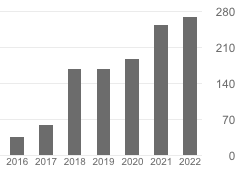
\includegraphics[height=30pt]{scholar-cit.png}

Names of students I supervise(d) are prepended with symbol \student{}.


\iffalse
\subsectionTitle{Under review}

% 2024 %%%%%%%%%%%%%%%%%%%%%%%%%%%%%%%%%%%%%%%%%%%%%%%%%%%%%%%%%%%%%%%%%%%%%%%%%%%%%%%%%
\begin{pubs}

\wsentry
	{}
	{\student{} Cuong Tran, Zarreen Reza, {\bf Ferdinando Fioretto}}
  	{On the unintended fairness effects of Low Rank Approximation in Large Language Models}
	{\procACL, 2024}
	{}
	
\wsentry
	{}
	{\student{} Razane Tajeddine, Ajinkya Mulay, Tudor Cebere, {\bf Ferdinando Fioretto}}
  	{From Adversarial Robustness to Differential Privacy and Back}
	{\procUAI, 2024}
	{}

\wsentry
	{}
	{\student{} James Kotry, \student{} My H.~Dinh, {\bf Ferdinando Fioretto}}
  	{End-to-End Optimization and Learning with Ordered Weighted Averages}
	{\procUAI, 2024}
	{}

\wsentry
	{}
	{\student{} Jacob K Christopher, {\bf Ferdinando Fioretto}}
  	{Projected Generative Diffusion Models for Constraint Satisfaction}
	{\procICML, 2024}
	{}
\wsentry
	{}
	{Khang Tran, {\bf Ferdinando Fioretto}, Issa Khalil, My T. Thai, Linh Thi Xuan Phan, Hai Phan}
  	{Achieving Fairness Certification with Differential Privacy}
	{\procICML, 2024}
	{}

\wsentry
	{}
	{\student{} Saswat Das, Marco Romanelli, {\bf Ferdinando Fioretto}}
	{Disparate Impact on Group Accuracy of Linearization for Private Inference}
	{\procICML, 2024}
	{}

\wsentry
	{}
	{Sree Harsha Nelaturu, Nishaanth Kanna Ravichandran, \student{} Cuong Tran, Sara Hooker, {\bf Ferdinando Fioretto}}
	{On The Fairness Impacts of Hardware Selection in Machine Learning}
	{\procICML, 2024}
	{}

\wsentry
	{}
	{Prakhar Ganesh, \student{} Cuong Tran, Reza Shokri, {\bf Ferdinando Fioretto}}
	{The Data Minimization Principle in Machine Learning}
	{\procFAccT, 2024}
	{}

\wsentry
	{}
	{\student{} My H.~Dinh, \student{} James Kotary, {\bf Ferdinando Fioretto}}
	{Learning Fair Ranking Policies via Differentiable Optimization of Ordered Weighted Averages}
	{\procFAccT, 2024}
	{}

\wsentry
	{}
	{\student{} James Kotary, \student{} Vincenzo Di Vito, \student{} Jacob K Christopher, Pascal Van Hentenryck, {\bf Ferdinando Fioretto}}
	{Learning Joint Models of Prediction and Optimization}
	{\procIJCAI, 2024}
	{}

\wsentry
	{}
	{\student{Cuong Tran}, Keyu Zhu, {\bf Ferdinando Fioretto}, Pascal Van Hentenryck}
	{Fairness Increases Adversarial Vulnerability}
	{\procIJCAI, 2024}
	{https://arxiv.org/abs/2211.11835}
\end{pubs}

\subsectionTitle{Refereed Conferences or Journal Papers}
\fi

\begin{pubs}
%{\nemph{Refereed Conferences or Journal Papers}}&\nemph{\rule{0.5\linewidth}{0.5pt}}\\[1em]
% 2024 %%%%%%%%%%%%%%%%%%%%%%%%%%%%%%%%%%%%%%%%%%%%%%%%%%%%%%%%%%%%%%%%%%%%%%%%%%%%%%%%%
% {\nemph{2020}}&\nemph{\rule{0.5\linewidth}{0.5pt}}\\[1em]

\wsentry
	{124}
	{\student{} James Kotary, {\bf Ferdinando Fioretto}}
	{Learning Constrained Optimization with Deep Augmented Lagrangian Methods}
	{\venue{CoRR abs}/2403.03454, 2024}
	{https://arxiv.org/abs/2403.03454}

\wsentry
	{123}
	{\student{}My H. Dinh, \student{} James Kotary, {\bf Ferdinando Fioretto}}
	{End-to-End Learning for Fair Multiobjective Optimization Under Uncertainty}
	{\venue{CoRR abs}/2402.07772, 2024}
	{https://arxiv.org/abs/2402.07772}

\wsentry
	{122}
	{\student{} Jacob K Christopher, {\bf Ferdinando Fioretto}}
  	{Projected Generative Diffusion Models for Constraint Satisfaction}
	{\venue{CoRR abs}/2402.03559, 2024}
	{https://arxiv.org/abs/2402.03559}

\wsentry
	{121}
	{\student{} Saswat Das, Marco Romanelli, {\bf Ferdinando Fioretto}}
	{Disparate Impact on Group Accuracy of Linearization for Private Inference}
	{\venue{CoRR abs}/2402.03629, 2024}
	{https://arxiv.org/abs/2402.03629}

\wsentry
	{120}
	{\student{} My H.~Dinh, \student{} James Kotary, {\bf Ferdinando Fioretto}}
	{Learning Fair Ranking Policies via Differentiable Optimization of Ordered Weighted Averages}
	{\venue{CoRR abs}/2402.05252, 2024}
	{https://arxiv.org/abs/2402.05252}

\confentry
	{119}
	{{\bf Ferdinando Fioretto}, Keyu Zhu, Pascal Van Hentenryck, \student{} Saswat Das and Christine Task}
  	{Finding $\epsilon$ and $\delta$ of Traditional Disclosure Control Systems}
	{\procAAAI, 2024}
	{https://arxiv.org/abs/2301.12204}
	{23.75\%}

\wsentry
	{118}
	{\student{James Kotary}, \student{Jacob Christopher}, \student{My H Dinh},
	and {\bf Ferdinando Fioretto}}
	{Analyzing and Enhancing the Backward-Pass Convergence of Unrolled Optimization}	
	{\venue{CoRR abs}/2301.12047, 2024}
	{https://arxiv.org/abs/2301.12047}


% 2023 %%%%%%%%%%%%%%%%%%%%%%%%%%%%%%%%%%%%%%%%%%%%%%%%%%%%%%%%%%%%%%%%%%%%%%%%%%%%%%%%%
% {\nemph{2020}}&\nemph{\rule{0.5\linewidth}{0.5pt}}\\[1em]
\wsentry
	{117}
	{\student{} Sree Harsha Nelaturu, \student{} Nishaanth Kanna Ravichandran, \student{} Cuong Tran, Sara Hooker, and {\bf Ferdinando Fioretto}}
	{On The Fairness Impacts of Hardware Selection in Machine Learning}	
	{\venue{CoRR abs}/2312.03886, 2023}
	{https://arxiv.org/abs/2312.03886}

\journalentry
	{116}
	{Mostafa Mohammadian, Kyri Baker, \textbf{Ferdinando Fioretto}}
	{Gradient-Enhanced Physics-Informed Neural Networks for Power Systems Operational Support}
	{Electric Power Systems Research, pages 109551, 2023}
	{https://www.sciencedirect.com/science/article/abs/pii/S0378779623004406}

\confentry
	{115}
	{\student{Cuong Tran} and {\bf Ferdinando Fioretto}}
	{Data Minimization at Inference Time}
	{\procNeurIPS, 2023}
	{https://arxiv.org/abs/2305.17593}
	{23\%}

\wsentry
	{114}
 	{Vladimir Dvorkin and {\bf Ferdinando Fioretto}}
  	{Price-Aware Deep Learning for Electricity Markets}
  	{Tackling Climate Change with Machine Learning, at NeurIPS 2023}
  	{https://arXiv.org/abs/2308.01436}

\confentry
	{113}
	{\student{My H. Dinh}, {\bf Ferdinando Fioretto}, Mostafa Mohammadian, and Kyri Baker}
	{An Analysis of the Reliability of AC Optimal Power Flow Deep Learning Proxies}
	{IEEE PES Innovative Smart Grid Technologies, 2023}
	{https://arxiv.org/abs/2111.11168}
	{unknown}

\confentry 
	{112} %{IJCAI}
	{\student{James Kotary}, \student{My H. Dinh}, {\bf Ferdinando Fioretto}}
	{Folded Optimization for End-to-End Model-Based Learning}
	{\procIJCAI, 2023}
	{https://arxiv.org/abs/2301.12047}
	{15\%}

\confentry
    {111} %{IJCAI}
	{\student{James Kotary}, \student{Vincenzo Di Vito}, {\bf Ferdinando Fioretto}, Pascal Van Hentenryck}
	{SF-PATE: Scalable, Fair, and Private Aggregation of Teacher Ensembles}
    {\procIJCAI, 2023}
	{https://arxiv.org/abs/2204.05157}
    {15\%}

\confentry
    {110} %{IJCAI}
	{\student{Cuong Tran}, \student{Keyu Zhu}, {\bf Ferdinando Fioretto}}
	{End-to-End Combinatorial Ensemble Learning}
    {\procIJCAI, 2023}
	{http://arxiv.org/abs/2211.00251}
    {15\%}

\confentry
    {109} %{IJCAI}
	{\student{Cuong Tran}, {\bf Ferdinando Fioretto}}
	{On the Fairness Impacts of Private Ensembles Models}
    {\procIJCAI, 2023}
	{http://arxiv.org/abs/2109.08630}
    {15\%}

\wsentry
	{108} %{PES}
	{Terrence W.K. Mak, {\bf Ferdinando Fioretto}, Pascal Van Hentenryck}
	{Load Encoding for Learning AC-OPF}
	{Proceedings of the \venue{IEEE PES General Meeting (PES)}, 2023}
	{https://arxiv.org/abs/2101.03973}

\confentry
    {107} %{AAMAS}
	{\student{James Kotary}, \student{Vincenzo Di Vito}, {\bf Ferdinando Fioretto}}
	{End-to-End Optimization and Learning for Multiagent Ensembles}
    {\procAAMAS, 2023}
	{http://arxiv.org/abs/2211.00251}
    {40\%}

\wsentry
	{106}
	{Jayanta Mandi, \student{James Kotary}, Senne Berden, Maxime Mulamba, Victor Bucarey, Tias Guns, {\bf Ferdinando Fioretto}} 
	{Decision-Focused Learning: Foundations, State of the Art, Benchmark and Future Opportunities}
	{\venue{CoRR abs}/2307.13565, 2023}
	{https://arxiv.org/abs/2307.13565}

\wsentry
	{105}
	{Khang Tran, {\bf Ferdinando Fioretto}, Issa Khalil, My T. Thai, NhatHai Phan} 
	{FairDP: Certified Fairness with Differential Privacy}
	{\venue{CoRR abs}/2305.16474, 2023}
	{https://arxiv.org/abs/2305.16474}

\wsentry 
	{104}%{ArXiv}
	{Keyu Zhu, {\bf Ferdinando Fioretto}, Pascal Van Hentenryck, Saswat Das, Christine Task}
	{Privacy and Bias Analysis of Disclosure Avoidance Systems}
	{\venue{CoRR abs}/2301.12204, 2023}
	{https://arxiv.org/abs/2301.12204}

\wsentry 
	{103}%{ArXiv}
	{\student{My H. Dinh}, {\bf Ferdinando Fioretto}}
	{Context-Aware Differential Privacy for Language Modeling}
	{\venue{CoRR abs}/2301.12288, 2023}
	{https://arxiv.org/abs/2301.12288}


% 2022 %%%%%%%%%%%%%%%%%%%%%%%%%%%%%%%%%%%%%%%%%%%%%%%%%%%%%%%%%%%%%%%%%%%%%%%%%%%%%%%%%

\journalentry
	{102} %{JAIR}
	{Khoi D.~Hoang, \textbf{Ferdinando Fioretto}, Ping Hou, William Yeoh, Makoto Yokoo, Roie Zivan}
	{Proactive Dynamic Distributed Constraint Optimization Problems}
	{\JAIR, (73), pages 179-225, 2022}
	{https://www.jair.org/index.php/jair/article/view/13499}
\confentryAwd
	{101} %{NeurIPS}
	{\student{Cuong Tran}, {\bf Ferdinando Fioretto}, Jung-Eun Kim, 
	\student{Rakshit Naidu}}
	{Pruning has a disparate impact on model accuracy}
	{\procNeurIPS, 2022}
	{http://arxiv.org/abs/2205.13574}
	{25.6\%} %48
	{Lightning Talk (Spotlight)}
	{(Typically assigned to $\sim$3\% out of all paper submissions (10,411, in 2022))}
\confentry
	{100} %{IJCAI}
	{Keyu Zhu, {\bf Ferdinando Fioretto}, Pascal Van Hentenryck}
	{Post-processing of Differentially Private Data: A Fairness Perspective}
	{\procIJCAI, 2022}
	{http://arxiv.org/abs/2202.09425}	
	{15\%}
\confentry
	{99} %{IJCAI}
	{{\bf Ferdinando Fioretto}, \student{Cuong Tran}, Keyu Zhu, Pascal Van Hentenryck}
	{Differential Privacy and Fairness in Decisions and Learning Tasks: A Survey}
	{\procIJCAI, 2022}
	{http://arxiv.org/abs/2202.08187}	
	{18\% (survey track)}
\confentryAwd
	{98} %{IJCAI}
	{{\bf Ferdinando Fioretto}}
	{Integrating Machine Learning and Optimization to Boost Decision Making}
	{\procIJCAI, 2022}
	{https://web.ecs.syr.edu/~ffiorett/files/papers/Fioretto-IJCAI22-EC.pdf}	
	{Invited}
	{Early Career Spotlight}
	{(Accompanying paper)}
\confentry
	{97} %{WWW}
	{\student{James Kotary}, {\bf Ferdinando Fioretto}, Pascal Van Hentenryck, Ziwei Zhu}
	{End-to-end Learning for Fair Ranking Systems}
	{\procWWW, 2022}
	{http://arxiv.org/abs/2111.10723}	
	{17\%}	
\confentry
	{96} %{AAAI} 
	{\student{James Kotary}, {\bf Ferdinando Fioretto}, Pascal Van Hentenryck}
	{Fast Approximations for Job Shop Scheduling: A Lagrangian Dual Deep Learning Method}
	{\procAAAI, 2022}
	{http://arxiv.org/abs/2110.06365}
	{15\%}
\confentry
	{95} %{PMAPS}
	{Lesia Mitridati, Emma Romei, Gabriela Hug, {\bf Ferdinando Fioretto}}
	{Differentially-Private Heat and Electricity Markets Coordination}
	{\procPMAPS, 2022}
	{https://arxiv.org/abs/2201.10634}
	{unknown} 
\confentry
	{94} %{PMAPS}
	{Mostafa Mohammadian, Kyri Baker, \student{My H.~Dinh}, {\bf Ferdinando Fioretto}}
	{Learning Solutions for Intertemporal Power Systems Optimization with Recurrent Neural Networks}
	{\procPMAPS, 2022}
	{https://ieeexplore.ieee.org/document/9810638}
	{unknown}
% \end{pubs}
% \begin{pubs}
\journalentry
	{93} %{AI Mag.}
	{{\bf Ferdinando Fioretto}, et al.} 
	{Reports of the Workshops Held at the 2022 AAAI Conference on Artificial Intelligence}
	{{\bf AI Magazine}, 2022}
	{https://interactiveaimag.org/updates/reports/reports-of-the-workshops-held-at-the-2022-aaai-conference-on-artificial-intelligence/}
\wsentryAwd
	{92} %{PPAI}
	{\student{Cuong Tran}, \student{My H.~Dinh}, {\bf Ferdinando Fioretto}}
	{A Fairness Analysis on Private Aggregation of Teacher Ensembles}
	{\venue{AAAI Workshop on Privacy Preserving Artificial Intelligence 
		(PPAI)--at AAAI}, 2022}
	{http://arxiv.org/abs/2109.08630}
	{Spotlight Paper}
\wsentry 
	{91}%{ArXiv}
	{\student{Cuong Tran}, Keyu Zhu, {\bf Ferdinando Fioretto}, Pascal Van Hentenryck}
	{Fairness Increases Adversarial Vulnerability}
	{\venue{CoRR abs}/2211.11835, 2022}
	{https://arxiv.org/abs/2211.11835}
\wsentry
	{90}%{ArXiv}
	{Mostafa Mohammadian, Kyri Baker, {\bf Ferdinando Fioretto}}
	{Gradient-Enhanced Physics-Informed Neural Networks for Power Systems Operational Support}
	{\venue{CoRR abs}/2206.10579, 2022}
	{https://arxiv.org/abs/2206.10579}
\wsentry 
	{89}%{ArXiv}
	{Sawinder Kaur, {\bf Ferdinando Fioretto}, Asif Salekin}
	{Deadwooding: Robust Global Pruning for Deep Neural Networks} 
	{\venue{CoRR abs}/2202.05226, 2022}
	{http://arxiv.org/abs/2202.05226}


% 2021 %%%%%%%%%%%%%%%%%%%%%%%%%%%%%%%%%%%%%%%%%%%%%%%%%%%%%%%%%%%%%%%%%%%%%%%%%%%%%%%%%
\journalentry
	{88} %{AIJ}
		{\textbf{Ferdinando Fioretto}, Pascal Van Hentenryck, Keyu Zhu}
		{Differential Privacy of Hierarchical Census Data: An Optimization Approach}
		{\AIJ, (296), pages 103475, 2021}
		{https://www.sciencedirect.com/science/article/pii/S0004370221000266}
\journalentryAwd
	{87} %{IEEE-TPS}
		{Vladimir Dvorkin, {\bf Ferdinando Fioretto}, Pascal Van Hentenryck, Pierre Pinson, Jalal Kazempour}
		{Differentially Private Optimal Power Flow for Distribution Grids}
		{\TPS, 36(3), pages 2186--2196, 2021}
		{https://ieeexplore.ieee.org/document/9226144}
		{Best IEEE TPS paper award}
		{(given to 8 out of all TPS papers published in 2019--2021)}
\confentry 
	{86} %{NeurIPS}
	{\student{Cuong Tran}, \student{My H. Dinh}, {\bf Ferdinando Fioretto}}
	{Differentially Private Deep Learning under the Fairness Lens}
	{\procNeurIPS, 2021}
	{https://arxiv.org/pdf/2106.02674.pdf}
	{26\%} % 9122
\confentry 
	{85} %{NeurIPS}
	{\student{James Kotary}, {\bf Ferdinando Fioretto}, Pascal Van Hentenryck}
	{Learning Hard Optimization Problems: A Data Generation Perspective}
	{\procNeurIPS, 2021}
	{https://arxiv.org/pdf/2106.02674.pdf}
	{26\%} % 9122
\confentryAwd 
	{84} %{IJCAI}
	{\student{Cuong Tran}, {\bf Ferdinando Fioretto}, Pascal Van Hentenryck, \student{Zhiyan Yao}}
	{Decision Making with Differential Privacy under the Fairness Lens}
	{\procIJCAI, 560--566, 2021}
	{https://www.ijcai.org/proceedings/2021/78}
	{13.9\%} %4,204/587
	{2022 Caspar Bowden PET Award}
	{(Selected among all papers about Privacy Enhancing Technologies published in international conferences between 2020--2022.)}
\confentry 
	{83} %{IJCAI}
	{\student{James Kotary}, {\bf Ferdinando Fioretto}, Pascal Van Hentenryck, Bryan Wilder}
	{End-to-End Constrained Optimization Learning: A Survey}
	{\procIJCAI, 4475--4482, 2021}
	{https://www.ijcai.org/proceedings/2021/610}
	{30.1\%}
\confentry 
	{82} %{AAAI}
	{Keyu Zhu, Pascal Van Hentenryck, {\bf Ferdinando Fioretto}}
	{Bias and Variance of Post-processing in Differential Privacy}
	{\procAAAI, 11177--11184, 2021}
	{https://ojs.aaai.org/index.php/AAAI/article/view/17333}
    {21.0\%} %  7,911/1,692
\confentry 
	{81} %{AAAI}
	{\student{Cuong Tran}, {\bf Ferdinando Fioretto}, Pascal Van Hentenryck}
	{Differentially Private and Fair Deep Learning: A Lagrangian Dual Approach}
	{\procAAAI, 9932--9939, 2021}
	{https://ojs.aaai.org/index.php/AAAI/article/view/17193}
    {21.0\%} %  7,911/1,692
\confentry
    {80} %{AAMAS}
    {\student{Anudit Nagar}, \student{Cuong Tran}, {\bf Ferdinando Fioretto}}
    {A Privacy-Preserving and Accountable Multi-agent Learning Framework}
    {\procAAMAS, 1605--1606, 2021}
    {https://dl.acm.org/doi/10.5555/3463952.3464174}
    {40\%}
\confentry
	{79} %{CP}
	{\bf Ferdinando Fioretto}
	{Constrained-based Differential Privacy}
	{\procCP, 1868--8969, 2021}
	{https://drops.dagstuhl.de/opus/volltexte/2021/15293/}
	{Invited}	
\confentry 
	{78} %{PowerTech}
	{Vladimir~Dvorkin, {\bf Ferdinando Fioretto}, Pascal Van Hentenryck, Jalal~Kazempour, Pierre~Pinson}
	{Differentially Private Optimal Power Flow for Distribution Grids}
	{\venue{IEEE PowerTech}, 2021}
	{https://ieeexplore.ieee.org/document/9226144}
	{N/A} %4,204/587
\journalentry
	{77} %{AI Mag.}
	{{\bf Ferdinando Fioretto}, et al.} 
	{Reports of the Workshops Held at the 2021 AAAI Conference on Artificial Intelligence}
	{{\bf AI Magazine}, 2021}
	{https://interactiveaimag.org/updates/reports/reports-of-the-workshops-held-at-the-2021-aaai-conference-on-artificial-intelligence/}
\wsentry
	{76} %{TPDP}
	{\student{Cuong Tran}, {\bf Ferdinando Fioretto}}
	{Decision Making with Differential Privacy under the Fairness Lens}
	{\venue{Theory and Practice of Differential Privacy (TPDP) -- at ICML}, 2021}
	{https://tpdp.journalprivacyconfidentiality.org/2021/}
\wsentry
	{75} %{OptLMAS}
	{\student{Anudit Nagar}, \student{Cuong Tran}, {\bf Ferdinando Fioretto}}
	{A Privacy-Preserving and Accountable Multi-agent Learning Framework}
	{\venue{International Workshop on Learning and Optimization 
 		   in Multi-Agent Systems (OPTLearnMAS)--at AAMAS}, 2021}
	{https://optlearnmas21.github.io/}
\wsentry
	{74} %{PPAI}
	{\student{Cuong Tran}, {\bf Ferdinando Fioretto}, Pascal Van 	Hentenryck}
	{Differentially Private and Fair Deep Learning: A Lagrangian Dual Approach}
	{\venue{AAAI Workshop on Privacy Preserving Artificial Intelligence 
		(PPAI)--at AAAI}, 2021}
	{https://arxiv.org/abs/2009.12562}
\wsentry 
	{73}%{ArXiv}
	{\student{My H.~Dinh}, {\bf Ferdinando Fioretto}, Mostafa Mohammadian, Kyri Baker}
	{Towards Understanding the Unreasonable Effectiveness of Learning AC-OPF Solutions}
	{\venue{CoRR abs}/2111.11168, 2021}
	{http://arxiv.org/abs/2111.11168}
\wsentry 
	{72}%{ArXiv}
	{\student{Cuong Tran}, \student{My H.~Dinh}, \student{Kyle Beiter}, {\bf Ferdinando Fioretto}}
	{A Fairness Analysis on Private Aggregation of Teacher Ensembles}
	{\venue{CoRR abs}/2109.08630, 2021}
	{http://arxiv.org/abs/2109.08630}
\wsentry % (NeruIPS-21)
	{71}%{ArXiv}
	{\student{Cuong Tran}, \student{My H.~Dinh}, {\bf Ferdinando Fioretto}}
	{Differentially Private Deep Learning under the Fairness Lens}
	{\venue{CoRR abs}/2106.02674, 2021 ({\bf extended NeurIPS-21 version})}
	{http://arxiv.org/abs/2106.02674}
\wsentry 
	{70}%{ArXiv}
	{\student{Anudit Nagar}, \student{Cuong Tran}, {\bf Ferdinando Fioretto}}
	{A Privacy-Preserving and Trustable Multi-agent Learning Framework}
	{\venue{CoRR abs}/2106.01242, 2021. ({\bf extended AAMAS-21 version})}
	{https://arxiv.org/abs/2106.01242}
\wsentry % (IJCAI-21 )
	{69}%{ArXiv}
	{\student{James Kotary}, {\bf Ferdinando Fioretto}, Pascal Van Hentenryck, Bryan Wilder}
	{End-to-End Constrained Optimization Learning: A Survey}
	{\venue{CoRR abs}/2103.16378, 2021. ({\bf extended IJCAI-21 version})}
	{https://arxiv.org/abs/2103.16378}
\wsentry 
	{68}%{ArXiv}
	{Terrence W.K. Mak, {\bf Ferdinando Fioretto}, Pascal VanHentenryck}
	{Load Embeddings for Scalable AC-OPF Learning}
	{\venue{CoRR abs}/2101.03973, 2021}
	{https://arxiv.org/abs/2101.03973}
\journalentry
	{67} %{AI Mag.}
	{{\bf Ferdinando Fioretto}, et al.} 
	{Reports of the Workshops Held at the 2020 International Association for the Advancement of Artificial Intelligence Conference on Web and Social Media}
	{{\bf AI Magazine},  41(4) 2020}
	{https://ojs.aaai.org/index.php/aimagazine/article/view/7486}
\wsentry 
	{66} %{INFORMS}
	{{\bf Ferdinando Fioretto}, \student{Cuong Tran}, Pascal Van Hentenryck}
	{Lagrangian Duality for Constrained Deep Learning}
	{\venue{INFORMS}, 2020}
	{http://meetings2.informs.org/wordpress/annual2020/}
\wsentry 
	{65} %{INFORMS}
	{Lesia Mitridati, {\bf Ferdinando Fioretto}, Pascal Van Hentenryck}
	{Differential Privacy For Stackelberg Games: An Application To Gas And Electricity Markets}
	{\venue{INFORMS}, 2020}
	{http://meetings2.informs.org/wordpress/annual2020/}
\wsentry 
	{64}%{ArXiv} 
	{Keyu Zhu, Pascal Van Hentenryck, {\bf Ferdinando Fioretto}}
	{Bias and Variance of Post-processing in Differential Privacy}
	{\venue{CoRR abs}/2010.04327, 2020 ({\bf extended AAAI-21 version})}
	{https://arxiv.org/abs/2010.04327}
\wsentry
	{63}%{ArXiv} 
	{Minas Chatzos, {\bf Ferdinando Fioretto}, Terrence W.K.~Mak, Pascal Van Hentenryck}
	{High-Fidelity Machine Learning Approximations of Large-Scale Optimal Power Flow}
	{\venue{CoRR abs}/2006.16356, 2020}
	{https://arxiv.org/abs/2006.16356}
\wsentry
	{62}%{ArXiv} 
	{Vladimir Dvorkin, {\bf Ferdinando Fioretto}, Pascal Van Hentenryck, Jalal Kazempour, Pierre Pinson}
	{Differentially Private Convex Optimization with Feasibility Guarantees}
	{\venue{CoRR abs}/2006.12338, 2020}
	{https://arxiv.org/abs/2006.12338}


% 2020 %%%%%%%%%%%%%%%%%%%%%%%%%%%%%%%%%%%%%%%%%%%%%%%%%%%%%%%%%%%%%%%%%%%%%%%%%%%%%%%%%

\journalentry
	{61} %{IEEE-TSG} 
		{{\bf Ferdinando Fioretto}, Terrence W.K.~Mak, Pascal Van Hentenryck}
		{Differential Privacy for Power Grid Obfuscation}
		{\TSG, 11(2), pages 1356--1366, 2020}
		{https://ieeexplore.ieee.org/document/8809257}
\journalentryAwd
	{60}	%{IEEE-TPS}
		{Terrence W.K.~Mak, {\bf Ferdinando Fioretto}, \student{Lyndon Shi}, Pascal Van Hentenryck}
		{Privacy-Preserving Power System Obfuscation: A Bilevel Optimization Approach}
		{\TPS, 35(2), pages 1627--1637, 2020}
		{https://ieeexplore.ieee.org/document/8854890}
		{Best IEEE TPS paper award}
		{(given to 7 out of all TPS papers published in 2018--2020)}
\confentry
		{59} %{ECML}
		{{\bf Ferdinando Fioretto}, Pascal Van Hentenryck, Terrence W.K. Mak, \student{Cuong Tran}, Federico Baldo, Michele Lombardi} 
		{A Lagrangian Dual Framework for Deep Neural Networks with Constraints}
		{\procECML, 18--135, 2020}
		{https://arxiv.org/abs/2001.09394}
		{19\%}
\confentry
		{58} %{IJCAI}
		{{\bf Ferdinando Fioretto}, Lesia Mitridati, Pascal Van Hentenryck}
		{Differential Privacy Stackebelg Games}
		{\procIJCAI, 3480--3486, 2020}
		{https://www.ijcai.org/proceedings/2020/0481.pdf}
	    {12.6\%}
\confentryAwd
		{57} %{IJCAI}
		{{\bf Ferdinando Fioretto}, Pascal Van Hentenryck}
		{OptStream: Releasing Time Series Privately}
		{\procIJCAI, 5135--5139, 2020}
	    {https://www.ijcai.org/proceedings/2020/722}
		{invited}
		{Invited to the IJCAI journal track}{}	
\confentry
		{56} %{PSCC}
		{Terrence W.K.~Mak, {\bf Ferdinando Fioretto}, Pascal Van Hentenryck}
		{Privacy-Preserving Obfuscation for Distributed Power Systems}
		{\procPSCC, 2020}
		{https://arxiv.org/abs/1910.04250}
	    {$\sim$30\%} %  7,737/1591
\confentry
		{55} %{AAAI}
		{{\bf Ferdinando Fioretto}, Terrence W.K.~Mak, Pascal Van Hentenryck}
		{Predicting AC Optimal Power Flows: Combining Deep Learning and Lagrangian Dual Methods}
	  	{\procAAAI, pages 630--637, 2020}
	  	{https://ojs.aaai.org//index.php/AAAI/article/view/5403}
	    {20.6\%} %  7,737/1591
\confentry
	{54} %{PRIMA}
    {Atena Tabakhi, William Yeoh, {\bf Ferdinando Fioretto}}
    {The Smart Appliance Scheduling Problem: A Bayesian Optimization Approach}
    {\procPRIMA, 100--115, 2020}
    {https://link.springer.com/chapter/10.1007\%2F978-3-030-69322-0\_7}
    {38.0\%} % 19/50

% 2019 %%%%%%%%%%%%%%%%%%%%%%%%%%%%%%%%%%%%%%%%%%%%%%%%%%%%%%%%%%%%%%%%%%%%%%%%%%%%%%%%%
\journalentryAwd
	{53}	%{JAIR}
	{{\bf Ferdinando Fioretto}, Pascal Van Hentenryck}
	{OptStream: Releasing Time Series Privately}
	{\JAIR, (65) pages 423--456, 2019}
	{https://www.jair.org/index.php/jair/article/view/11583}
	{Invited to IJCAI 2020 journal track}
	{}
\journalentryAwd
	{52}	%{IA}
	{{\bf Ferdinando Fioretto}, Agostino Dovier, Enrico Pontelli}
	{Distributed Multi-Agent Optimization for Smart Grids and Home Automation}
	{\venue{Intelligenza Artificiale (IA)},  12 (2), pages: 67--87, 2019}
	{https://content.iospress.com/articles/intelligenza-artificiale/ia180037}
	{Best 2018 Thesis in Artificial Intelligence (AI*IA)}
	{(Accompanying paper)}
\confentry
	{51} %{AAMAS}
	{{\bf Ferdinando Fioretto}, Pascal Van~Hentenryck}
	{Privacy-Preserving Federated Data Sharing}
  	{\procAAMAS, pages 638--646, 2019}
  	{https://dl.acm.org/doi/abs/10.5555/3306127.3331750}
	{24\%} % 189/781
\confentry
	{50} %{IJCAI}
	{{\bf Ferdinando Fioretto}, Terrence W.K.~Mak, Pascal Van Hentenryck}
	{Privacy-Preserving Obfuscation of Critical Infrastructure Networks}
  	{\procIJCAI, pages 1086--1092, 2019}
  	{https://www.ijcai.org/proceedings/2019/0152.pdf}
    {17.9\%} %  4,752/850
\confentryAwd
	{49} %{CP}
	{{\bf Ferdinando Fioretto}, Pascal Van Hentenryck}
	%\href{https://web.ecs.syr.edu/~ffiorett/files/papers/cp19.pdf}
	{Differential Privacy of Hierarchical Census Data: An Optimization Approach} 
	{\procCP, pages 639--655, 2019}
	{https://link.springer.com/chapter/10.1007/978-3-030-30048-7\_37}
	{37\%}
	{Invited to Constraint journal}
	{(selected papers -- declined)}
\wsentry 
	{48} %{OptMAS}
	{Khoi Hoang, {\bf Ferdinando Fioretto}, William Yeoh, Enrico Pontelli, Roie Zivan}
	{A Large Neighboring Search Schema for Multi-Agent Optimization} 
	{\venue{International Workshop on Optimization 
 		   in Multi-Agent Systems (OPTMAS)--at AAMAS}, 2019}
	{https://www2.isye.gatech.edu/~fferdinando3/cfp/OPTMAS19/}
\wsentry
	{47}%{ArXiv} 
	{{\bf Ferdinando Fioretto}, Terrence W.K.~Mak, Pascal Van Hentenryck}
	{Predicting AC Optimal Power Flows: Combining Deep Learning and Lagrangian Dual Methods}
	{\venue{CoRR abs}/1909.10461, 2019 ({\bf extended AAAI-20 version})}
	{https://arxiv.org/abs/1909.10461}
\wsentry
	{46}%{ArXiv} 
	{{\bf Ferdinando Fioretto}, Terrence W. K. Mak, Pascal Van Hentenryck}
	{Privacy-Preserving Obfuscation of Critical Infrastructure Networks} 
	{\venue{CoRR abs}/1905.09778, 2019 ({\bf extended IJCAI-19 version})}
	{https://arxiv.org/abs/1905.09778}


% 2018 %%%%%%%%%%%%%%%%%%%%%%%%%%%%%%%%%%%%%%%%%%%%%%%%%%%%%%%%%%%%%%%%%%%%%%%%%%%%%%%%%

\journalentry
	{45}	%{JAIR}
	{{\bf Ferdinando Fioretto}, Enrico Pontelli, William Yeoh}
	{Distributed Constraint Optimization Problems and Applications: A Survey}
	{\JAIR, 61, pages 623--698, 2018} 
	{https://arxiv.org/abs/1602.06347}
\journalentry 
	{44}	%{AI Matters}
	{{\bf Ferdinando Fioretto}, William Yeoh}
	{AI Buzzwords Explained: Distributed Constraint Optimization Problems}
	{\venue{AI Matters}, 3 (4), pages 8--13, 2018}
	{https://sigai.acm.org/static/aimatters/3-4/AIMatters-3-4-04-Fioretto.pdf}
\journalentry 
	{43}	%{Constraints}
	{{\bf Ferdinando Fioretto}, Enrico Pontelli, William Yeoh, Rina Dechter}
	{Accelerating Exact and Approximate Inference for (Distributed) Discrete Optimization with GPUs}
	{\venue{Constraints}, 23 (1), pages 1--43, 2018}
	{https://link.springer.com/article/10.1007/s10601-017-9274-1}
\confentry 
	{42} %{PRIMA}
	{{\bf Ferdinando Fioretto}, Hong Xu, Sven Koenig, TK Satish Kumar}
 	{Solving Multiagent Constraint Optimization Problems on the Constraint Composite Graph}
	{\procPRIMA, pages 106--122, 2018}
	{https://link.springer.com/chapter/10.1007/978-3-030-03098-8\_7}
    {26\%} % 27/103
\confentry
	{41} %{AAMAS}
  	{{\bf Ferdinando Fioretto}, Chansoo Lee, Pascal Van Hentenryck}
  	{Constrained-based Differential Privacy for Private Mobility} 
  	{\procAAMAS, pages 1405--1413, 2018}
  	{https://dl.acm.org/doi/abs/10.5555/3237383.3237910}
    {25\%} % 151/597
\confentry 
	{40} %{CP}
	{Khoi Hoang, {\bf Ferdinando Fioretto}, William Yeoh, Enrico Pontelli, Roie Zivan}
	{A Large Neighboring Search Schema for Multi-Agent Optimization}
	{\procCP, pages 688--706, 2018}
	{https://link.springer.com/chapter/10.1007/978-3-319-98334-9\_44}
    {33\%} % 3/9 (in this track)
\confentry 
	{39} %{CPAIOR}
	{{\bf Ferdinando Fioretto}, Pascal Van Hentenryck}
	{Constrained-based Differential Privacy: Releasing Optimal Power Flow Benchmarks Privately} 
	{\procCPAIOR, pages 215--231, 2018}
	{https://link.springer.com/chapter/10.1007/978-3-319-93031-2\_15}
    {48\%}
\confentry
	{38} %{ISIAM}
	{{\bf Ferdinando Fioretto}, Hong Xu, Sven Koenig, TK Satish Kumar}
	{Constraint Composite Graph-Based Lifted Message Passing for Distributed Constraint Optimization Problems}
	{\procISIAM, 2018}
	{https://speakerdeck.com/xuphys/constraint-composite-graph-based-lifted-message-passing-for-distributed-constraint-optimization-problems}
	{N/A}
\wsentry
	{37} %{OptMAS}
	{{\bf Ferdinando Fioretto}, Hong Xu, Sven Koenig, TK Satish Kumar}
	{Solving Multiagent Constraint Optimization Problems on the Constraint Composite Graph} 
	{\venue{International Workshop on Optimisation in Multi-Agent Systems 
	(OptMAS)--at AAMAS}, 2018}
	{~}

% 2017 %%%%%%%%%%%%%%%%%%%%%%%%%%%%%%%%%%%%%%%%%%%%%%%%%%%%%%%%%%%%%%%%%%%%%%%%%%%%%%%%%

% {\nemph{2017}}&\nemph{\rule{0.5\linewidth}{0.5pt}}\\[1em]
\journalentryAwd
	{36} %{LNCS}
	{\student{William Kluegel}, \student{Muhammad A.~Iqbal}, {\bf Ferdinando Fioretto}, William Yeoh, Enrico Pontelli}
	{A Realistic Dataset for the Smart Home Device Scheduling Problem for DCOPs}
	{\emph{Lecture Notes in Computer Science (LCNS)}, LNCS, volume 10643 pages 125--142, Springer, 2017}
	{https://link.springer.com/chapter/10.1007\%2F978-3-319-71679-4\_9}
	{Visionary Paper Award}
	{(AAMAS workshop series)}
\journalentry
	{35} %{LNBIP}
	{Moinul M.P.~Chowdhury, Russell Y.~Folk, {\bf Ferdinando Fioretto}, Christopher Kiekintveld, William Yeoh}
	{Investigation of Learning Strategies for the SPOT Broker in Power TAC}
	{\emph{AgentMediated Electronic Commerce: Designing Trading Strategies and Mechanisms for Electronic Markets}, volume 271 of Lecture Notes in Business Information Processing, 
	    pages 96–111, Springer, 2017}
    {https://link.springer.com/chapter/10.1007\%2F978-3-319-54229-4\_7}
\confentry 
	{34} %{AAMAS}
	{{\bf Ferdinando Fioretto}, William Yeoh, Enrico Pontelli, Ye Ma, Satishkumar J.~Ranade}
	{A Distributed Constraint Optimization (DCOP) Approach to the Economic Dispatch with Demand Response}
	{\procAAMAS, pages  999--1007, 2017}
	{https://dl.acm.org/doi/10.5555/3091125.3091267}
	{25\%}%{\it 137/550 = 25\%}.
\confentry 
	{33} %{AAMAS}
	{{\bf Ferdinando Fioretto},  William Yeoh, Enrico Pontelli}
	{A Multiagent System Approach to Scheduling Devices in Smart Homes}
	{\procAAMAS, pages 981--989, 2017} 
	{https://dl.acm.org/doi/10.5555/3091125.3091265}
	{25\%}%{\it 137/550 = 25\%}
\confentry
	{32} %{AAMAS} 
	{Khoi Hoang, Ping Hou, {\bf Ferdinando Fioretto}, Makoto Yokoo, William Yeoh, Roie Zivan}
	{Infinite-Horizon Proactive Dynamic DCOPs}
	{\procAAMAS, pages 212--220, 2017}
	{https://dl.acm.org/doi/10.5555/3091125.3091160}
	{25\%}%{\it 137/550 = 25\%}.
\confentry 
	{31} %{CP}
	{Atena M.~Tabakhi, Tiep Le, {\bf Ferdinando Fioretto}, William Yeoh}
	{Preference Elicitation for DCOPs}
	{\procCP, pages 278--296, 2017}
	{https://link.springer.com/chapter/10.1007/978-3-319-66158-2\_18}
	{43\%}%{\it 50+4/(137+17) = 25\%}.
\wsentry
	{30} %{OptMAS}	
	{William Kluegel, Muhammad Aamir Iqbal, {\bf Ferdinando Fioretto}, William Yeoh, Enrico Pontelli}
	{A Realistic Dataset for the Smart Home Device Scheduling Problem for DCOPs}
	{\venue{International Workshop on Optimisation in Multi-Agent Systems (OPTMAS)--at AAMAS}, 
	2017}
	{~}	
\wsentry
	{29} %{AISGSB}
	{{\bf Ferdinando Fioretto},  William Yeoh, Enrico Pontelli}
	{A Multiagent System Approach to Scheduling Devices in Smart Homes}
	{\venue{Workshop on AI for Smart Grids and Smart Buildings (AISGSB)--at AAAI}, 2017}
	{~}

% 2016 %%%%%%%%%%%%%%%%%%%%%%%%%%%%%%%%%%%%%%%%%%%%%%%%%%%%%%%%%%%%%%%%%%%%%%%%%%%%%%%%%

% {\nemph{2016}}& \nemph{\rule{0.5\linewidth}{0.5pt}}\\[1em]
\confentry 
	{28} %{AAMAS}
	{Khoi Hoang, {\bf Ferdinando Fioretto}, Ping Hou, Makoto Yokoo, William Yeoh, Roie Zivan}
	{Proactive Dynamic Distributed Constraint Optimization Problems} 
	{\procAAMAS, pages 597--605, 2016}
	{https://www.ifaamas.org/Proceedings/aamas2019/pdfs/p2411.pdf}
	{25\%}%{\it 137/550 = 25\%}.
\confentry 
	{27} %{AAMAS}
	{Tiep Le, {\bf Ferdinando Fioretto}, William Yeoh, Enrico Pontelli, Tran Cao Son} 
	{ER-DCOPs: A Framework for Distributed Constraint Optimization Problems With Uncertainty} 
	{\procAAMAS,	pages 606--614, 2016}
	{https://dl.acm.org/doi/10.5555/2936924.2937014}
	{25\%}%{\it 137/550 = 25\%}.
\confentry 
	{26} %{AAAI}
	{{\bf Ferdinando Fioretto}, William Yeoh, Enrico Pontelli}
	{Multi-Variable Agent Decompositions for DCOPs}
	{\procAAAI, pages 2480--2486, 2016}
	{https://dl.acm.org/doi/10.5555/3016100.3016246}
	{26\%}%{\it 549/2132 = 26\%}.
\confentry
	{25} %{CP} 
	{{\bf Ferdinando Fioretto}, William Yeoh, Enrico Pontelli}
	{A Dynamic Programming-Based MCMC Framework for Solving DCOPs with GPUs}
	{\procCP, pages 813--831,	2016}
	{https://link.springer.com/chapter/10.1007/978-3-319-44953-1\_51}
	{35\%}%{\it 50+4/(137+17) = 34\%}.
\wsentry
	{24} %{MPREF} 
	{Atena M.~Tabakhi, {\bf Ferdinando Fioretto}, William Yeoh}
	{A Preliminary Study on Preference Elicitation in DCOPs for Scheduling Devices in Smart Buildings}
	{\venue{10th Workshop on Advances in Preference Handling (MPREF)--at IJCAI}, 2016}
	{~}
\wsentry 
	{23} %{TADA}
	{Porag Chowdhury, Russell Y. Folk, {\bf Ferdinando Fioretto}, Christopher Kiekintveld, William Yeoh}
	{Investigation of Learning Strategies for the SPOT Broker in Power TAC}
  	{\venue{International Workshop on Agent Mediated Electronic Commerce and Trading Agents Design and Analysis
	(AMEC/TADA)--at AAMAS}, 2016}
	{~}
\wsentry 
	{22} %{AISGSB}
	{Khoi Hoang, {\bf Ferdinando Fioretto}, Ping Hou, Makoto Yokoo, William Yeoh, Roie Zivan}
	{Proactive Dynamic DCOPs} 
	{\venue{Workshop on AI for Smart Grids and Smart Buildings (AISGSB)--at AAAI}, 2016}
	{~}	

% 2015 %%%%%%%%%%%%%%%%%%%%%%%%%%%%%%%%%%%%%%%%%%%%%%%%%%%%%%%%%%%%%%%%%%%%%%%%%%%%%%%%%

% {\nemph{2015}}&\nemph{\rule{0.5\linewidth}{0.5pt}}\\[1em]
\journalentry 
	{21}	%{TOMACS}
	{{\bf Ferdinando Fioretto}, Agostino Dovier, Enrico Pontelli}
	{Constrained Community-based Gene Regulatory Network Inference}
	{\venue{ACM Transactions on Modeling and Computer Simulation (TOMACS)}, 25 (2), pages 11:1--11:26, 2015}
	{https://dl.acm.org/doi/10.1145/2688909}
\confentry
	{20} %{CP}
	{{\bf Ferdinando Fioretto}, Tiep Le, Enrico Pontelli, William Yeoh, Tran Cao Son}
	{Exploiting GPUs in Solving (Distributed) Constraint Optimization Problems with Dynamic Programming}
	{\procCP, pages 121--139, 2015}
	{https://dl.acm.org/doi/10.5555/3102787.3102797}
	{49\%}%{\it  39/80 = 49\%}.
\confentry
	{19} %{AAMAS}
	{{\bf Ferdinando Fioretto}, Federico Campeotto, Agostino Dovier, Enrico Pontelli, William Yeoh}
	{Large Neighborhood Search with Quality Guarantees for Distributed Constraint Optimization Problems}
	{\procAAMAS, pages 1835--1836, 2015}
	{https://dl.acm.org/doi/10.5555/2772879.2773461}
	{46\%}
\confentry
	{18} %{AAMAS}
	{{\bf Ferdinando Fioretto}, William Yeoh, Enrico Pontelli}
	{Multi-Variable Agents Decomposition for DCOPs to Exploit Multi-Level Parallelism}
	{\procAAMAS, pages 1823--1824, 2015}
	{https://dl.acm.org/doi/10.5555/2772879.2773455}
	{46\%}
\confentry
	{17} %{AAMAS}
	{{\bf Ferdinando Fioretto}}
	{Exploiting the Structure of Distributed Constraint Optimization Problems} 
	{\procAAMAS, pages 2007--2008, 2015}
	{https://dl.acm.org/doi/10.5555/2772879.2773549}
	{N/A}
\confentry
	{16} %{AAAI}
	{{\bf Ferdinando Fioretto}} 
	{Exploiting the Structure of Distributed Constraint Optimization Problems}
	{\procAAAI,  pages 4233--4234, 2015}
	{https://www.aaai.org/ocs/index.php/AAAI/AAAI15/paper/view/9293}
	{N/A}
\wsentry
	{15} %{OptMAS} 
	{{\bf Ferdinando Fioretto}, Federico Campeotto, Agostino Dovier, Enrico Pontelli, William Yeoh}
	{Large Neighborhood Search with Quality Guarantees for Distributed Constraint Optimization Problems} 
	{In \venue{International Workshop on Optimization in Multi-Agent Systems (OptMAS)-- at AAMAS}, 2015}
	{~}
\wsentry 
	{14} %{OptMAS}
	{{\bf Ferdinando Fioretto}, Tiep Le, William Yeoh, Enrico Pontelli, Tran Cao Son}
	{Improving DPOP with Branch Consistency for Solving Distributed Constraint Optimization Problems}
	{In \venue{International Workshop on Optimization in Multi-Agent Systems (OptMAS)-- at AAMAS}, 2015}
	{~}

% <2014 %%%%%%%%%%%%%%%%%%%%%%%%%%%%%%%%%%%%%%%%%%%%%%%%%%%%%%%%%%%%%%%%%%%%%%%%%%%%%%%%%
\confentry 
	{13} %{ECAI}
	{($\alpha$-$\beta$) 
	Federico Campeotto, Agostino Dovier, {\bf Ferdinando Fioretto}, Enrico Pontelli}
	{A GPU Implementation of Large Neighborhood Search for Solving Constraint Optimization Problems} 
	{\procECAI, pages 189--194, 2014}
	{https://dl.acm.org/doi/10.5555/3006652.3006685}
	{28\%}
\confentry
	{12} %{CP}
	{{\bf Ferdinando Fioretto}, Tiep Le, William Yeoh, Enrico Pontelli, Tran Cao Son}
	{Improving DPOP with Branch Consistency for Solving Distributed Constraint Optimization Problems}
	{\procCP, pages 307--323, 2014}
	{https://link.springer.com/chapter/10.1007\%2F978-3-319-10428-7\_24}
	{50\%}
\confentry
	{11} %{PADL}
	{($\alpha$-$\beta$) 
	Federico Campeotto, Alessandro Dal Pal\`{u}, Agostino Dovier, {\bf Ferdinando Fioretto}, Enrico Pontelli}
	{Exploring the Use of GPUs in Constraint Solving}
	{\procPADL, pages 152--167, 2014}
	{https://link.springer.com/chapter/10.1007\%2F978-3-319-04132-2\_11}
	{55\%}
\confentry 
	{10} %{AAMAS}
	{{\bf Ferdinando Fioretto}, Federico Campeotto, Luca Da Rin Fioretto, William Yeoh, Enrico Pontelli} 
	{GD-Gibbs: A GPU-based Sampling Algorithm for Solving Distributed Constraint Optimization Problems} %(Extended Abstract)". 
	{\procAAMAS, pages 1339--1340, 2014}
	{https://dl.acm.org/doi/10.5555/2615731.2617462}
	{46\%}
\journalentry
	{9}	%{JAIR}
	{($\alpha$-$\beta$)\footnote{Author list is order alphabetically.} 
	Federico Campeotto, Alessandro Dal Pal\`{u}, Agostino Dovier,  {\bf Ferdinando Fioretto}, Enrico Pontelli}
	{A Constraint Solver for Flexible Protein Models}
	{\JAIR, 48, pages 953--1000, 2013}
	{https://www.jair.org/index.php/jair/article/view/10856}
\confentryAwd
	{8} %{CMSB}
	{{\bf Ferdinando Fioretto}, Enrico Pontelli} 
	{Constraint Programming in Community-based Gene Regulatory Network Inference} 
	{\procCMSB, pages 135--149, 2013}
	{https://link.springer.com/chapter/10.1007\%2F978-3-642-40708-6\_11}
	{55\%}
	{Best Student Paper Award}{}
\confentry 
	{7} %{CP}
	{($\alpha$-$\beta$) 
	Federico Campeotto, Alessandro Dal Pal\`{u}, Agostino Dovier, {\bf Ferdinando Fioretto}, Enrico Pontelli}
	{A Filtering Technique for Fragment Assembly-based Proteins Loop Modeling with Constraints} 
	{\procCP, pages 850--866, 2012}
	{https://link.springer.com/chapter/10.1007\%2F978-3-642-33558-7\_61}
	{36\%}
\confentry
	{6} % {Neuroscience}
	{Michael R. Best, {\bf Ferdinando Fioretto}, Alessandro Dal Pal\`{u}, Enrico Pontelli, Tran Son, TuShun R. Powers, Elba E. Serrano}
	{The role of secondary and tertiary structure prediction in determining the function of novel genes found in Xenopus Leavis}
	{\venue{Neuroscience}, 2011, (518.20/ZZ45)}{}
	{N/A}
\wsentry 
	{5} %{WCB}
	{($\alpha$-$\beta$) 
	Federico Campeotto, Alessandro Dal Pal\`{u}, Agostino Dovier, {\bf Ferdinando Fioretto}, Enrico Pontelli} 
  	{Experimenting with FIASCO for protein structure prediction}
	{\venue{Workshop on Constraint Based Methods for Bioinformatics (WCB)--at CP}, 2014}
	{~}
\wsentry 
	{4} %{ParSeachOpt}
	{($\alpha$-$\beta$) Federico Campeotto, Alessandro Dal Pal\`{u}, Agostino Dovier, {\bf Ferdinando Fioretto}, Enrico Pontelli}
	{Towards a complete constraint solver on GPU}
	{In \venue{Workshop on Parallel Methods for Search \& Optimization (ParSearchOpt)--at ECAI}, 2014}
	{~}
\wsentry 
	{3} %{WCB}
	{{\bf Ferdinando Fioretto}, Enrico Pontelli}
	{Community-based Gene Regulatory Network Inference via Constraint Programming}
	{\venue{Workshop on Constraint Based Methods for Bioinformatics (WCB)--at CP}, 2013}
	{~} 
\wsentry
	{2} %{WCB} 
	{($\alpha$-$\beta$) 
	Federico Campeotto, Alessandro Dal Pal\`{u}, Agostino Dovier, {\bf Ferdinando Fioretto}, Enrico Pontelli}
	{Protein Loop Modelling via Constraints and Fragment Assembly}
	{\venue{Workshop on Constraint Based Methods for Bioinformatics (WCB)--at CP}, 2012}
	{~} 
\wsentry 
	{1} %{WCB}
	{($\alpha$-$\beta$) 
	Michael R. Best, Kabi Bhattarai, Federico Campeotto, Alessandro Dal Pal\`{u}, Hung Dang, Agostino Dovier, {\bf Ferdinando Fioretto}, Federico Fogolari, Tiep Le, Enrico Pontelli}
		{Introducing FIASCO: Fragment-based Interactive Assembly for protein Structure prediction with COnstraints}
 	 {\venue{Workshop on Constraint Based Methods for  Bioinformatics (WCB)--at CP}, 2011}
  	{~}
\end{pubs}  
	%!TEX root= cvFioretto.tex
%Section: Scholarships and additional info
\sectionTitle{Teaching}{}%{\faMortarBoard}

% \begin{experiences}
%   \teach
%     {Spring 2021} {Security and Privacy of Machine Learning (CS 700)}{Syracuse University}
%     {4.93/5.00 (median 5.00)}
%   \teach
%     {Fall 2021} {Introduction to Artificial Intelligence (CIS 467)}{Syracuse University}
%     {4.38/5.00 (median 5.00)}
%   \teach
%     {Spring 2021} {Security and Privacy of Machine Learning (CS 700)}{Syracuse University}
%     {4.46/5.00 (median 5.00)}
%   \teach
%     {Fall 2020} {Introduction to Artificial Intelligence (CIS 467)}{Syracuse University}
%     {4.56/5.00 (median 5.00)}
%   \teach
%     {Spring 2020} {Security and Privacy of Machine Learning (CS 700)}{Syracuse University}
%     {4.55/5.00 (median 5.00)}
% \end{experiences}


\begin{experiences}
  \multicolumn{2}{l}{\textbf{Artificial Intelligence (CS 4710)}, 
                         \textit{University of Virginia}}\\[0.35em]
  \textbf{Fall 2023} & \textsc{Course Evaluation: } {4.33(class), 4.5(instructor)/5.00}\\[0.35em]

  \multicolumn{2}{l}{\textbf{Security and Privacy of Machine Learning (CS 700)}, 
                         \textit{Syracuse University}}\\[0.35em]
  \textbf{Spring 2020} & \textsc{Course Evaluation: } {4.55/5.00 (median 5.00)}\\[0.35em]
  \textbf{Spring 2021} & \textsc{Course Evaluation: } {4.46/5.00 (median 5.00)}\\[0.35em]
  \textbf{Spring 2022} & \textsc{Course Evaluation: } {4.93/5.00 (median 5.00)}\\
  \emptySeparator

  \multicolumn{2}{l}{\textbf{Introduction to Artificial Intelligence (CIS 467)}, 
                         \textit{Syracuse University}}\\[0.35em]
  \textbf{Fall 2020} & \textsc{Course Evaluation: } {4.56/5.00 (median 5.00)}\\[0.35em]
  \textbf{Fall 2021} & \textsc{Course Evaluation: } {4.48/5.00 (median 5.00)}\\[0.35em]
  \textbf{Fall 2022} & \textsc{Course Evaluation: } {4.45/5.00 (median 5.00)}\\[0.35em]
  \textbf{Fall 2023} & \textsc{Course Evaluation: } {4.15/5.00 (median 5.00)}\\
  \emptySeparator

  \multicolumn{2}{l}{\textbf{Discrete Mathematics (CS 375)}, 
                         \textit{Syracuse University}}\\[0.35em]
   \textbf{Spring 2023} & \textsc{Course Evaluation: } {4.60/5.00 (median 5.00)}\\[0.35em]


\end{experiences}

\sectionTitle{Mentoring}{}%{\faGroup}

\subsection*{PhD Students}
\begin{itemize}
  \item \textbf{James Kotary} ({\sc Syracuse University}, CISE) 
  \hfill{\em Fall 2020 -- current}\\
  {\sc Research}: Integration of Deep Learning and Optimization.
  %Current Position: \textit{Same}

  \item \textbf{Vincenzo Di Vito} ({\sc Syracuse University} CISE)
  \hfill{\em Fall 2022 -- current}\\
  {\sc Research:} Physics Informed Machine Learning.
  
  \item \textbf{My Dinh} ({\sc Syracuse University} CISE) 
  \hfill{\em Spring 2021 -- current}\\
  {\sc Research}: Deep Learning, Optimization, Fairness.
  %Current Position: \textit{Same}

  \item \textbf{Saswat Das} ({\sc University of Virginia} CS)
  \hfill{\em Fall 2023 -- current}\\
  {\sc Research:} Responsible AI, Differential Privacy.

  \item \textbf{Jacob K.~Christopher} ({\sc University of Virginia} CS)
  \hfill{\em Fall 2023 -- current}\\
  {\sc Research:} Responsible AI in Generative Models.

  \item \textbf{Cuong Tran} ({\sc Syracuse University}, CISE) 
  \hfill{\em Spring 2020 -- Spring 2023}\\
  {\sc Research}: Differential Privacy and Fairness.\\
  {\sc Dissertation Title:} The Interplay between Privacy and Fairness in
  Learning and Decision-making Problems\\
  {\sc Next position:} Postdoc at University of Virginia 
\end{itemize}
\medskip

\subsection*{Postdocs}
\begin{itemize}
    \item \textbf{Cuong Tran} ({\sc University of Virginia}, CS) 
  \hfill{\em Sep 2023 -- Mar 2024}\\
  {\sc Research}: Data Minimization, Fairness in Large Language Models.

    \item \textbf{Razan Tajeddine} ({\sc Visitor at University of Virginia}, CS) 
  \hfill{\em Sep 2023 -- Mar 2024}\\
  {\sc Research}: Differential Privacy and Fairness.
\end{itemize}

\subsection*{MS Students (including Interns/Visitor)}
\begin{itemize}
  \item \textbf{Klaus Peng} ({\sc University of Virginia}) \hfill{\em Fall 2023}\\
  {\sc Research:} Causality.
  
  \item \textbf{Jacob Kennedy Christopher} ({\sc Syracuse University}) \hfill{\em Spring 2023}\\
  {\sc Research:} Differentiable Optimiztion.\\
  {\sc Next position:} PhD student at \textit{University of Virginia}.

  \item \textbf{St John Grimbly} ({\sc University of South Africa}) \hfill{\em Spring 2023}\\
  {\sc Research:} Causality and Fairness.\\
  {\sc Next position:} PhD student at \textit{University of South Africa}.

  \item \textbf{Yehya Farhat} ({\sc SU}) \hfill{\em Fall 2022}\\
  {\sc Proposed Thesis:} Surrogate ML models for optimization.

  \item \textbf{Rakshit Naidu} ({\sc CMU}) \hfill{\em Summer 2022}\\
  {\sc Research:} Privacy and Fairness in ML.\\
  {\sc Next position:} PhD student at \textit{Carnegie Mellon University}

  % \item \textbf{Mainul Islam} ({\sc IIT Kharagpur}) \hfill{\em Summer 2022}\\
  % {\sc Research:} Natural Language Processing.

  % \item   \textbf{Harini Suresh} ({\sc  UCLA}) \hfill{\em 2022}\\
  % {\sc Research:} Federated Learning.

  \item \textbf{Pratik Paranjape} ({\sc Syracuse University}, CISE) 
  \hfill{\em Summer 2020}\\
  {\sc Research}: Generating datasets for preference elicitation.\\
  First job after graduation: \textit{Developer at OthersideAI}

  \item \textbf{Pavan Kumar Vaddineni}  ({\sc Syracuse University}, CISE), \hfill{\em Spring 2020}\\
  {\sc Research}: Explainable and Fair Learning.\\
  First job after graduation: \textit{Same}

  \item \textbf{William Kluegel} (New Mexico State University, CS) \hfill{\em 2016 -- 2018} \\
  {\sc Research}: \textit{Optimization and Preferences Elicitation for Smart Home Devices.}\\
  First job after graduation: \textit{Sandia National Labs}
\end{itemize}
\medskip

\subsection*{BS and High-School Students}
  \textbf{Eric Nguyen} (UVA, 2023-2024) % sampling and DP
  \textbf{Joonhyuk Ko} (UVA, 2024) % sampling and DP
  \textbf{Catherine Smolka} (Deep Run High School, VA, 2023-2024), 
  \textbf{Pranav Putta} (GaTech, Summer 2023) [REU],
  \textbf{Winston Tsui} (SU, Summer 2023),
  \textbf{Zhongquan Cheng} (SU, Summer 2023), 
  %%
  \textbf{Adya Parida} (SU, Fall 2022) [REU], 
  \textbf{Deniz Gursoy} (Fayetteville High School, Summer 2022), 
  \textbf{Saswat Das} (ITS, Summer 2022), 
  \textbf{Utsav Pathak} (Alliance University, Bengaluru, Summer 2022),
  \textbf{Daiwei Shen} (Northwestern, Summer 2022),
  \textbf{Sunisth Kumar} (Bennett University, Summer 2022),
  %%
  \textbf{Kyle Beiter} (SU, Summer 2021) [REU],  %REU
  \textbf{Shantanu Jhaveri} (USC, Summer 2021) [REU], % REU
  \textbf{Dayong Gu} (SU, Summer 2021),
  \textbf{Guoliang Chen} (SU, Summer 2021),
  \textbf{Pradyumn Yadav} (SU, Summer 2021),
  %%
  \textbf{Anudit Nagar} (SU, Summer 2020 -- Current), 
  \textbf{Zhiyan Yao} (SU, Summer 2020 -- Current),
  \textbf{Zifei Lu} (SU, Summer 2020),
  \textbf{Thomas Montfort} (SU, Summer 2020),
  \textbf{Cong Liu} (SU, Summer 2020),
  \textbf{Lyndon Shi} (UMich, 2018)
  \textbf{Jiayu Chen} (UMich, 2018)
  \textbf{Eric Frechette} (NMSU, 2016).

\medskip

\subsection*{PhD Dissertation Committee}
\begin{itemize}
  \item \textbf{Guangtao Zheng}, ({\sc University of Virginia}) \hfill 2024
  \item \textbf{Dung Nguyen}, ({\sc University of Virginia}) \hfill 2023
  \item \textbf{Elena Long}, ({\sc University of Virginia}) \hfill 2023
  \item \textbf{Khang Tran}, ({\sc New Jersey Institute of Technology}) \hfill 2023
  \item \textbf{Keyu Zhu}, ({\sc Georgia Institute of Technology}) \hfill 2023
  \item \textbf{Adrià Fenoy Barcel}, ({\sc University of Verona}) \hfill 2023
  \item \textbf{Jeroen Fransman}, ({\sc Delft University of Technology}) \hfill 2022
  \item \textbf{Pegah Hozhabrierdi}, ({\sc Syracuse University}) \hfill 2022
  \item \textbf{Carlos Pinzon}, ({\sc École Polytechnique}) \hfill 2022
  \item \textbf{Baocheng Geng}, ({\sc Syracuse University}) \hfill 2021
  \item \textbf{Pranay Sharma}, ({\sc Syracuse University}) \hfill 2021
\end{itemize}
\medskip
	%!TEX root=cvFioretto.tex

\sectionTitle{Tutorials, Selected Invited Talks and Media Interviews}{}%{\faTv}%{\faMicrophone}

\begin{itemize}
  \item {\bf Keynote Talk}: {Privacy and Fairness in Societal Systems}\\
  {\em  Workshop on the Tradeoffs in Ethical AI, INRIA, France}
  \hfill{Novermber 2023}

  \item {\bf Invited Talk}: {Responsible AI: Privacy and Fairness in Decision Making and Learning Tasks}\\
  {\em  TOC FOR FAIRNESS, Simons Collaboration on the Theory of Algorithmic Fairness.}
  \hfill{November 2023}

  \item {\bf Panelist}: {Navigating the Frontiers of Artificial Intelligence}\\
  {\em  The Center for Politics, University of Virginia}
  \hfill{October 2023}

  \item {\bf Invited Talk}: {Optimization and Learning for Science and Engineering}\\
  {\em  Conference on Complex Systems 2023}
  \hfill{October 2023}

  \item {\bf Invited Talk}: {ML for Optimization and Optimization for ML}\\
  {\em  AI/ML Seminar Series, University of Virginia}
  \hfill{September 2023}

  \item {\bf Keynote Talk}: {The Unintended Societal Effects of Privacy in Decision and Learning Tasks}\\
  {\em  IJCAI-2023, International Workshop on Mining Actionable Insights from Social Networks}
  \hfill{August 2023}

  \item {\bf Invited Talk}: {End-to-end Constrained Optimization Learning}\\
  {\em  AC Summer School: Machine Learning for Constraint Programming}
  \hfill{July 2023}

  \item {\bf Invited Talk}: {Differential Privacy for Power Systems}\\
  {\em  DTU PES Summer School}
  \hfill{June 2023}

  \item {\bf Invited Talk}: {Optimization Proxies and Differentiable Optimization for Decision Making}\\
  {\em  MARS Seminar, Pacific Northwest National Laboratory (PNNL)}
  \hfill{June 2023}

  \item {\bf Invited Talk}: {Constrained-aware Machine Learning in Energy Systems}\\
  {\em  IEEE Power and Energy Society webinar series}
  \hfill{June 2023}

  \item {\bf Invited Talk}: {Responsible AI: Privacy and Fairness in Decision and Learning Tasks}\\
  {\em  UC San Diego}
  \hfill{April 2023}

  \item {\bf Panelist}: {ChatGPT: Charms and Challenges}\\
  {\em  Syracuse University}
  \hfill{April 2023}

  \item {\bf Invited Talk}: {Responsible AI: Privacy and Fairness in Decision and Learning Tasks}\\
  {\em  University of Virginia}
  \hfill{March 2023}

  \item {\bf Invited Talk}: {Constrained-Aware Machine Learning}\\
  {\em  Washington University in St.~Louis}
  \hfill{Feb 2023}

  \item {\bf Invited Talk}: {Differential Privacy for Power Systems}\\
  {\em  Los Alamos National Lab's 5th Grid Science Winter School and Conference}
  \hfill{Jan 2023}

  \item {\bf Invited Panelist}: {Algorithmic Fairness and its Intersections}\\
  \press{https://neurips.cc/virtual/2022/tutorial/55815}
  {\em Thirty-sixth Conference on Neural Information Processing Systems (NeurIPS)}
  \hfill{Dec 2022}

  \item {\bf Tutorial}: {End-to-end constrained optimization learning}\\
  \press{https://aixia2022.uniud.it/}{\em 21st International Conference of the Italian Association for Artificial Intelligence (AIxIA 2022)}
  \hfill{Dec 2022}

  \item {\bf Media Cover}: 
  {How network pruning can skew deep learning models}\\ 
  \press{https://www.sciencedaily.com/releases/2022/11/221102115535.htm}{{\em Science Daily}}~
  \press{https://techxplore.com/news/2022-11-network-pruning-skew-deep.html}{TechXplore}~
  \press{https://www.eurekalert.org/news-releases/970000}{AAAS EurekAlert}~
  \hfill {Nov 2022}

  \item {\bf Invited Talk}: {Disparate Impacts in Privacy-preserving Machine Learning}\\
  {\em Washington University in St.~Louis} \hfill{Nov 2022}
  % {\em University of Maryland, College Park}  \hfill {Nov 2022}
  %{\em New Jersey Institute of Technology}    \hfill {Dec 2022}

  \item {\bf Tutorial}: {Decision Focused Learning}\\
  \em{Dagstuhl seminar on Data-Driven Combinatorial Optimisation}
  \hfill{Oct 2022}

  \item {\bf Media Interview}: {Privacy and Fairness in AI}\\
  \press{https://news.syr.edu/blog/2022/08/03/professor-receives-award-for-outstanding-research-in-privacy-enhancing-technologies/}{Syracuse Media Report}~
  \press{https://artsci.nmsu.edu/news-events/2022/07/nmsu-alumnus-gains-international-recognition-for-research-on-privacy-and-fairness-in-ai.html}{NMSU News}
  \press{https://www.lcsun-news.com/story/news/education/nmsu/2022/09/03/nmsu-alum-gains-international-recognition-for-research-on-ai-privacy/65467086007/}{Sun News}
  \hfill Jul/Sep 2022

  \item {\bf Media Interview}: {Google Scholar Research Award}\\
  \press{https://news.syr.edu/blog/2022/06/22/two-professors-win-prestigious-google-research-scholar-awards/}{Syracuse Media Report}
  \hfill Jun 2022

  \item {\bf Tutorial}: {Impacts of Data Privacy and Equity on Public Policy}\\ 
  \press{https://www.youtube.com/watch?v=ersvD5Nja98&t=8s&ab_channel=FerdinandoFioretto}{\em ACM Conference on Fairness, Accountability, and Transparency (FAccT)}
  \hfill {Jun 2022}

  \item {\bf Invited Panelist}: Fostering the Use of AI for Power System Transformation\\
  \press{https://www.climatechange.ai/webinars}{\em Climate Change AI}
  \hfill Jun 2022

  \item {\bf Media Interview}: {NSF CAREER Award}\\
  \press{https://ecs.syracuse.edu/about/news/electrical-engineering-and-computer-science-professor-ferdinando-fioretto-receives-national-science-foundation-nsf-career-award}{Syracuse Media Report}
  \hfill Jun 2022

  \item {\bf Invited Talk}: End-to-end constrained deep learning optimization\\
  {\em Hall of Science (Kantar.com)} 
  \hfill Mar 2022

  \item {\bf Panelist}: {AAAI-22 DC - Career Panel}\\
  \press{https://aaai.org/Conferences/AAAI-22/doctoral-consortium-program/}{\em 36th AAAI Conference on Artificial Intelligence (AAAI)}
  \hfill {Feb 2022}

  \item {\bf Invited Talk}: {Privacy-preserving ML and decisions-making: uses and unintended disparate effects}\\
  \press{https://prisec-ml.github.io/}{\em PriSec-ML (virtual seminars)}
  \hfill {Feb 2022}

  \item {\bf Media Interview}:  {AI for Climate Change}\\ 
  \press{https://www.rainews.it/tgr/puglia/notiziari/index.html?/tgr/video/2021/12/ContentItem-4aae6540-8707-4a9f-8b6d-3ec515470539.html}
  %https://www.raiplay.it/programmi/playdigital}{RaiPlay} 
  {RaiNews}\hfill {Dec 2021}

  \item {\bf Popular Media Report}: ISSNAF Young Investigator Award \hfill\\
  \press{https://www.lavocedinewyork.com/people/nuovo-mondo/2021/12/10/issnaf-premia-i-migliori-giovani-ricercatori-italiani-in-usa-e-chiude-un-anno-di-nuovi-progetti/}{New York Voice}~
  \press{https://www.aise.it/comunit\%C3\%A0/issnaf-premia-i-migliori-giovani-ricercatori-italiani-negli-usa/169636/}{AISE}~
  \press{https://www.ilmattinodifoggia.it/news/cultura/56658/nando-fioretto-di-san-severo-tra-i-finalisti-del-premio-ai-giovani-scienziati-italiani-del-nord-america.html}{{\em Il Mattino}}~
  \press{https://startupitalia.eu/166650-20211126-dallai-alla-letteratura-i-ricercatori-italiani-che-innovano-in-nord-america}{{\em StartupItalia}}~
  \press{https://citymilano.com/2021/11/25/dalla-sostenibilita-globale-allinnovazione-nelle-scienze-umane-ecco-i-migliori-giovani-ricercatori-italiani-in-nord-america/}{{\em Zox}}~
  \press{https://www.puglianews24.eu/dalla-puglia-ad-harvard-per-studiare-i-geni-e-combattere-la-leucemia-62441.html}{{\em PugliaNews}}
  \hfill {Nov 2021}

  \item {\bf Invited Talk}:  {Deep Constraint Learning: Applications and Privacy Considerations}\\
  \press{https://www.youtube.com/watch?v=eyKhU3GzdYA&ab_channel=ISSNAF-ItalianScientistsandScholarsinNorthAmericaFoundation}{\em Italian Scientists \& Scholars in North America Foundation} 
  \hfill {Nov 2021}

  \item \textbf{Plenary Keynote Talk}: Constraint-based Differential Privacy\\
  \press{https://cp2021.lirmm.fr/submissions/1002}{\em The International Conference on Principle and Practice of Constraint Programming (CP 2021)}, 
  \hfill Oct 2021

  \item {\bf Popular Media Interview}: 
  {Deep Learning for Engineering Applications}\\ 
  \press{https://blum.vision/?lang=en}{{\em Blum News}} \hfill {Nov 2021}

  \item \textbf{Invited Talk}: 
  Privacy-Preserving Machine Learning: Uses and Unintended Disparate Effect\\
  {\em ASPI Seminar (Syracuse University)} 
  \hfill Sep 2021
	
  \item \textbf{Invited Talk}: 
  Differential Privacy and Machine Learning\\
  {\em SUPA ECS workshop for High School Teachers}
  \hfill May 2021

  % \item {\it Invited Talk, REsearch Exposure in Socially Relevant Computing}
  % \hfill {Apr 2021}

  \item {\bf Invited Talk}: Deep Constraint Learning for Critical Engineering Systems\\
  \press{https://www.youtube.com/watch?v=eyKhU3GzdYA&ab_channel=ISSNAF-ItalianScientistsandScholarsinNorthAmericaFoundation}{\em Italian Scientists \& Scholars in North America Foundation} 
  \hfill {Nov 2020}

  \item {\bf Tutorial}: {Tutorial on Multiagent Optimization}\\ 
  \press{https://www2.isye.gatech.edu/~fferdinando3/cfp/AAAI20/}{\em AAAI Conference on Artificial Intelligence (AAAI 2020)} 
  \hfill {Feb 2020}

  \item {\bf Media Cover}: {Multiagent Systems} \\
  \press{https://www.agendadigitale.eu/cultura-digitale/i-sistemi-multiagente-cosi-governiamo-lintelligenza-artificiale/}{NetworkDigital360} \hfill{Feb 2020}

  \item {\bf Invited Talk}: 
  Privacy-Preserving Artificial Intelligence\\
  {\em University of Parma (CS Dept)} 
  \hfill {Jun 2019}

  \item {\bf Tutorial}: {Tutorial on Multiagent Optimization for IoT Applications}\\ 
  \press{}{\em International Conference on Autonomous Agents and Multiagent Systems (AAMAS 2019)} 
  \hfill {May 2019}

  \item {\bf Invited Talk}: Differential Privacy for AI Applications\\
  {\em University of Southern California - Information Sciences Institute} \hfill {Jan 2019}\\
  {\em Michigan State University} \hfill {Feb 2019}

  \item {\bf Invited Talk}: Privacy Preserving Artificial Intelligence\\
  {\em Syracuse University} \hfill {Feb 2019}\\
  {\em Drexel University} \hfill {Feb 2019}\\
  {\em University of Arkansas} \hfill {Feb 2019}\\
  {\em Colorado State University} \hfill {Mar 2019}\\
  {\em University of Connecticut} \hfill {Mar 2019}
  % {\em University of New Mexico} \hfill {Mar 2019}

  %{\em Missouri University of Science and Technology} \hfill {Feb 2019}
  % {\em University of Denver} \hfill {Jan 2019}

	% \item {\it AI Lab Seminar}, University of Michigan (EECS Dept)
	% \hfill {Aug 2018}

   % \item {\it Invited Presentation}, 
	% Privacy in Machine Learning and Artificial Intelligence Workshop 
	% (ICML/IJCAI/AAMAS 2018)
	% \hfill {Jun 2018}

	% \item {\it AI Seminar}, University of Southern California Information Sciences Institute (USC ISI)
	% \hfill {Mar 2018}

	% \item {\bf Seminar}: Differential Privacy for AI Applications\\
	% {\em New Mexico State University} \hfill {Mar 2018}

	\item {\bf Tutorial}: {Tutorial on Constrained Multi-agent Optimization}\\
	\press{https://www2.isye.gatech.edu/~fferdinando3/cfp/AAAI20/}{\em AAAI Conference on Artificial Intelligence (AAAI 2018)} 
  	\hfill {Feb 2018}

	\item {\bf Plenary Keynote Talk}: 
	Distributed Constraint Optimization for Smart Energy Networks\\
    {\em Italian Conference on Artificial Intelligence (AI*IA 2017)}
	\hfill {Nov 2017}

	\item {\bf Invited Talk}: Distributed Constraint Optimization\\
	{\em Delft University (TU Delft)} \hfill {Apr 2016}\\
 	{\em University of Udine} \hfill {Apr 2016} \\ 
	{\em New Mexico State University} \hfill {Mar 2016}
	
	\item {\bf Invited Talk}: Large Neighboring Search for Distributed Constrained Optimization\\
	{\em Ben-Gurion University of the Negev} \hfill {Mar 2016}
\end{itemize}
 
	%\pagebreak
	%!TEX root= cvFioretto.tex
\newpage

%Section: Project
\sectionTitle{Research Grants and Gifts}{}%{\faFlask}
\begin{keywords}
\keywordsentry{\textbf{Summary}:}
{\underline{Total External}: \$2,848,003 %~~ (\$1,527,403 as PI) 
\hspace{8pt} \underline{Total Internal}: \$81,000}%
\end{keywords}


\begin{projects}
	\grantentrySinglePI
	{University of Virginia (Research Innovation Award)}
	{60,000}
	{Aug.~2024}{Jun.~2024}
	{Understanding and Mitigating Privacy Leakage Risks for Large Language Model Applications}
	{}
	{Ferdinando Fioretto and David Evans}

	\grantentrycoPI
	{National Science Foundation (CISE - RI)}
	{350,000}{600,000}
	{Aug.~2023}{Jun.~2026}
	{Collaborative Research: RI: Small: End-to-end Learning of Fair and Explainable Schedules for Court Systems}
	{https://www.nsf.gov/awardsearch/showAward?AWD_ID=2232054}
	{Ferdinando Fioretto (lead)}
	{Lauryn Gouldin}

	\grantentryPI
	{National Science Foundation (EECS - EPCN)}
	{260,000}{520,000}
	{Aug.~2023}{Jun.~2026}
	{Collaborative Research: Physics Informed Real-time Optimal Power Flow}
	{https://www.nsf.gov/awardsearch/showAward?AWD_ID=2242931}
	{Ferdinando Fioretto}

	\grantentrySinglePI
	{Amazon Research Awards AWS AI}
	{55,000}
	{Jan.~2023}{}
	{Toward Understanding the Unintended Disparate Impacts of  Private Machine Learning Systems}
	{~}
	{Ferdinando Fioretto}

	\grantentrySinglePI
	{National Science Foundation (CAREER, CISE - RI)}
	{515,403}
	{Mar.~2022}{Feb.~2027}
	{CAREER: End-to-end Constrained Optimization Learning}
	{https://www.nsf.gov/awardsearch/showAward?AWD_ID=2143706}
	{Ferdinando Fioretto}	
	
	\grantentrySinglePI
	{Google Research Scholar Award}
	{60,000}
	{Jul.~2022}{}
	{On the Equity of Differentially Private Decision Processes}
	{https://research.google/outreach/research-scholar-program/recipients/}
	{Ferdinando Fioretto}

	\grantentryPI
	{National Science Foundation (CISE - SaTC)}
	{281,000}{500,000}
	{Oct.~2021}{Sep.~2025}
	{Collaborative Research: SaTC: Core: Small: Privacy and Fairness in Critical Decision Making}
	{https://www.nsf.gov/awardsearch/showAward?AWD_ID=2133169}
	{Ferdinando Fioretto (lead)}

	\grantentryPI
	{National Science Foundation (CISE - RI)}
	{266,000}{500,000}
	{Oct.~2020}{Sep.~2024}
	{Collaborative Research: RI: Small: Deep Constrained Learning for Power Systems}
	{https://www.nsf.gov/awardsearch/showAward?AWD_ID=2007164}
	{Ferdinando Fioretto}

\grantentrycoPI
	{CUSE Program}
	{21,000}{21,000}
	{Jun.~2021}{May~2023}
	{On the Potential Perils of Fairness Algorithms in Decision Making and Learning Tasks}
	{}
	{Ferdinando Fioretto}
	{Sucheta Soundarajan}
\end{projects}

\vspace{-16pt}
\subsectionTitle{\hspace{-16pt}Travel and Service Grants}

\begin{projects}
	\grantentrySinglePI
	{National Science Foundation}
	{50,000}
	{May.~2024}{}
	{Conference: Artificial Intelligence Summer School for Computer Science and Operations Research Education}
	{~}
	{Lavanya Marla and Ferdinando Fioretto}

	\grantentrySinglePI
	{Artificial Intelligence Journal}
	{4,000}
	{Mar.~2024}{}
	{Student Support AU-SCORE 2024}
	{}
	{Ferdinando Fioretto and Lavanya Marla}

	\grantentrySinglePI
	{Artificial Intelligence Journal}
	{15,000}
	{Jan.~2023}{}
	{Student Support for AAMAS 2023}
	{}
	{Ana L. C. Bazzan and Ferdinando Fioretto}
\end{projects}

\begin{projects}
	\grantentrySinglePI
	{National Science Foundation}
	{25,000}
	{May.~2023}{}
	{Travel: Travel: Doctoral Mentoring Consortium at the 22nd International Conference on Autonomous Agents and Multiagent Systems}
	{~}
	{Ferdinando Fioretto}

	\grantentrySinglePI
	{Google}
	{5,000}
	{Feb.~2023}{}
	{Support for Scholarship awards to attend the 2023 AAAI Privacy Preserving AI workshop}
	{~}
	{Ferdinando Fioretto}

	\grantentrySinglePI
	{Google}
	{2,500}
	{Feb.~2022}{}
	{Support for Scholarship awards to attend the 2023 AAAI Privacy Preserving AI workshop}
	{~}
	{Ferdinando Fioretto}
\end{projects}

\iffalse
\subsectionTitle{Under review/in preparation}
\begin{projects}
	\grantentrySinglePI
	{Amazon Research Awards AWS AI}
	{70,000}
	{}{}
	{The Principle of Data Minimization in Machine Learning}
	{~}
	{Ferdinando Fioretto}

	\grantentrySinglePI
	{National Science Foundation (CISE - SaTC)}
	{1,200,000}
	{}{}
	{Collaborative Research: SaTC: Medium: Post-processing in Differential Privacy: 
	Understanding Bias, Variance, and Fairness of Downstream Decisions}
	{~}
	{Ferdinando Fioretto and Juba Ziani}

	\grantentrySinglePI
	{National Science Foundation (ENG - CIS)}
	{500,000}
	{}{}
	{End-to-End Learning for Planning Safe, Comfortable, and Equitable Bicycle Infrastructure}
	{~}
	{Xilei Zhao and Ferdinando Fioretto}

	\grantentrySinglePI
	{DARPA YFA}
	{1,000,000}
	{}{}
	{Towards Certifiable Constraint-aware Generative Models}
	{~}
	{Ferdinando Fioretto}

	\grantentrySinglePI
	{National Science Foundation (CISE - RI)}
	{600,000}
	{}{}
	{RI: Small: Constraint-aware Generative AI: Adhering to Constraints and Physical Principles}
	{~}
	{Ferdinando Fioretto}
	
	\grantentrySinglePI
	{UVA RIA (intramural)}
	{60,000}
	{}{}
	{Understanding and Mitigating Privacy Leakage Risks for Large Language Model Applications}
	{~}
	{Ferdinando Fioretto and David Evans}

	\grantentrySinglePI
	{DOE Early Career Research Program}
	{not yet determined}
	{}{}
	{(pre-proposal stage) Deep Learning for Optimization in Multi-scale Systems}
	{~}
	{Ferdinando Fioretto}
	
\end{projects}
\fi 
	%%!TEX root= cvFioretto.tex
%Section: Project


\subsectionTitle{\hspace{-16pt}Pending Grants Submissions}
\medskip

\begin{itemize}
	\item \textbf{\textsc{DOE EXPRESS}}, 
	(\$500,000)  \hfill \textsc{5/25}\\
	{\bf Project title:} {Transformers as Constrained Optimizers: Foundations, Efficiency, and In-Context Learning for Scientific AI}\\
	{\bf Role:} PI (with Hadi Daneshmand as coPI)

	\item \textbf{\textsc{DOE Early Career Research Program}}, 
	(\$875,000)  \hfill \textsc{4/25}\\
	{\bf Project title:} {Foundational Methods for Constrained Generative Modeling in Scientific Computing}\\
	{\bf Role:} PI

	\item \textbf{\textsc{Amazon Research Awards AWS AI}}, 
	(\$70,000) \hfill \textsc{04/25}\\
	{\bf Project title:} {Massively Accelerating Large Language Models Inferences through Speculative Diffusion Decoding}\\
	{\bf Role:} PI

	% \item \textbf{\textsc{University of Virginia, RIA}}, 
	% (\$60,000) \hfill \textsc{01/25}\\
	% {\bf Project title:} {Constraining Generative AI for Safe Embodied Robotic Agents}\\
	% {\bf Role:} PI (with Nicola Bezzo as coPI)

	\item \textbf{\textsc{National Science Foundations}}, 
	(\$600,000)  \hfill \textsc{3/25}\\
	{\bf Project title:} {Constrained Generation for Scientific and Engineering Applications}\\
	{\bf Role:} PI

	\item \textbf{\textsc{DARPA YFA}}, 
	(\$1,000,000)  \hfill \textsc{2/25}\\
	{\bf Project title:} {Constraint-Driven Generative AI for Grounded, Physics-informed, and Reliable Outputs}\\
	{\bf Role:} PI

	\item \textbf{\textsc{National Science Foundations}}, 
	(\$1,200,000) \hfill \textsc{08/24}\\
	{\bf Project title:} {Privacy and Fairness: From Data Collection to Downstream Decisions}\\
	{\bf Role:} PI (with Juba Ziani (Georgia Tech) as coPI)

	% \item \textbf{\textsc{CISCO}}, 
	% (\$100,000) \hfill \textsc{10/24}\\
	% {\bf Project title:} {Massively Accelerating Foundations Models through Speculative Diffusion Decoding}\\
	% {\bf Role:} PI

	\item \textbf{\textsc{CISCO}}, 
	(\$100,000) \hfill \textsc{10/24}\\
	{\bf Project title:} {Disclosure Audits for LLM-powered Agentic Systems}\\
	{\bf Role:} co-PI (with David Evans as PI)

	\item \textbf{\textsc{4VA Grants}}, 
	(\$30,000) \hfill \textsc{01/25}\\
	{\bf Project title:} {Towards Fair and Interpretable LLM-based Decision Systems}\\
	{\bf Role:} PI (with Ziwei Zhu as coPI)

	\item \textbf{\textsc{4VA Grants}}, 
	(\$30,000) \hfill \textsc{01/25}\\
	{\bf Project title:} {Dynamic LLM Benchmarks for Multimodal Social Intelligence}\\
	{\bf Role:} PI (with Jindong Wang as coPI)

	% \item \textbf{\textsc{3-Cavalliers, UVA}}, 
	% (\$80,000) \hfill \textsc{01/25}\\
	% {\bf Project title:} {Advancing Multi-Contrast Brain MRI with High-Resolution Generative Diffusion Models}\\
	% {\bf Role:} PI (with Craig Meyer and Mathews Jacob as coPIs)

	% \item \textbf{\textsc{University of Virginia (Research Innovation Award)}}
	% (\$60,000)
	% \hfill \textsc{8/24-7/25}\\
	% {\bf Project title:} \nemph{Understanding and Mitigating Privacy Leakage Risks for Large Language Model Applications}\\
	% {\bf Role:} PI (with David Evans as coPI)
\end{itemize}

(Several other grants are in preparation, including three NSF and one DOE proposals.)  
% In all proposals included here I play the primary role. I am also part of several other proposals being submitted where I 
% play a secondary role (as co-PI or senior personnel) and are not included in this list.)

\iffalse
\begin{projects}
	\grantentrySinglePI
	{Amazon Research Awards AWS AI}
	{70,000}
	{Oct.~2024}{(pending)}
	{Massively Accelerating Large Language Models Inferences through Speculative Diffusion Decoding}
	{~}
	{Ferdinando Fioretto}

	\grantentrycoPI
	{National Science Foundation}
	{1,200,000}
	{Jun 2024}{(pending)}
	{Privacy and Fairness: From Data Collection to Downstream Decisions}
	{~}
	{Ferdinando Fioretto}
	{Juba Ziani}

	\grantentrySinglePI
	{National Science Foundation}
	{600,000}
	{Dec.~2024}{(planned)}
	{Towards Certifiable Constraint-aware Generative Models}
	{~}
	{Ferdinando Fioretto}

	\grantentrycoPI
	{National Science Foundation (CISE - III)}
	{600,000}
	{Jan 2025}{(planned)}
	{Characterizing and Mitigating the Unintended Disparate Impacts of Constrained Machine Learning Systems}
	{~}
	{Ferdinando Fioretto}{David Evans}

	\grantentrycoPI
	{National Science Foundation}
	{600,000}
	{Jan.~2025}{(declined)}
	{SaTC: Understanding and Mitigating Disclosure Risks for Large Language Model Applications}
	{~}
	{Ferdinando Fioretto}{David Evans}

	\grantentrycoPI
	{National Science Foundation}
	{20,000,000}
	{May~2024}{(declined)}
	{Theme 3: AI Institute: A Vision for Leaping toward Artificial General Intelligence (LeapAI)}
	{~}
	{Aidong Zhang}
	{Henry Kautz, Sven Koenig, Heng Huang, Dinesh Manocha, Ming Lin, Madhav Marathe}

	\grantentrycoPI
	{DOE}
	{3,000,000}
	{May 2024}{(declined)}
	{E2P2: Energy Efficient Privacy Preserving Federated Learning}
	{~}
	{Kevin J. Barker}{Deepak Tosh}{Ferdinando Fioretto}

\end{projects}
\fi
	%!TEX root=cvFioretto.tex
%%%%%%%%%%%%%%%%%%%%%%%%%%%%%%%%%%%%%%%%%
% CV Fioretto
% Service
%	PC
%	Reviewer
%%%%%%%%%%%%%%%%%%%%%%%%%%%%%%%%%%%%%%%%%
\sectionTitle{Service}{}%{\faPencil}

\subsectionTitle{Conference Chair}
\begin{itemize}    
    \item {\bf International Conference on Principles and Practice of Constraint Programming (CP)}  \hfill{2022} \\
    {\em with Roie Zivan}
\end{itemize}

\subsectionTitle{Workshop Chair}
  \begin{itemize}
    \item 
    {\bf AAAI Workshop on Learnable Optimization (LEANOPT)}, at AAAI   \hfill{2024}
    \\{\em with Elias B. Khalil, Pascal Van Hentenryck, Jan Drgona, Draguna Vrabie, and Priya Donti}

    \item 
    {\bf Fifth AAAI Workshop on Privacy Preserving Artificial Intelligence (PPAI)}, at AAAI   \hfill{2024}
    \\{\em with Juba Ziani, Christine Task, and Niloofar Mireshghallah}

    \item
    {\bf Algorithmic Fairness through the lens of Time (AFT)}, at NeurIPS \hfill {2023}
    \\{\em with Awa Dieng, Miriam Rateike, and Golnoosh Farnadi}

    \item 
    {\bf Workshop on Optimization and Learning in Multi-Agent Systems}, at AAMAS \hfill{2023}
    \\{\em with Hau Chan, Jiaoyang Li, Filippo Bistaffa, and James Kotary}

    \item 
    {\bf Fourth AAAI Workshop on Privacy Preserving Artificial Intelligence (PPAI)}, at AAAI   \hfill{2023}
    \\{\em with Catuscia Palamidessi, and Pascal Van Hentenryck}

    \item
    {\bf Algorithmic Fairness through the lens of Causality and Privacy (AFCP)}, at NeurIPS \hfill {2022}
    \\{\em with Awa Dieng, Miriam Rateike, and Golnoosh Farnadi}

    \item 
    {\bf Workshop on Optimization and Learning in Multi-Agent Systems}, at AAMAS \hfill{2022}
    \\{\em with Hau Chan and Jiaoyang Li}

    \item 
    {\bf Third AAAI Workshop on Privacy Preserving Artificial Intelligence (PPAI)}, at AAAI   \hfill{2022}
    \\{\em with Aleksandra Korolova and Pascal Van Hentenryck}
    \item 
    {\bf AAAI Workshop on Machine Learning for Operational Research (ML4OR)}, at AAAI   \hfill{2022}
    \\{\em with Emma Frejinger, Elias Khalil, and Pashootan Vaezipoor}
    \item 
    {\bf Second AAAI Workshop on Privacy Preserving Artificial Intelligence (PPAI)}, at AAAI   \hfill{2021}
    \\{\em with Pascal Van Hentenryck and Richard W. Evans}
    \item 
    {\bf Workshop on Optimization and Learning in Multi-Agent Systems (OptLearnMAS)}, at AAMAS \hfill{2021}
    \\{\em with Amulya Yadev, Gauthier Picard, and Bryan Wilder}
    \item 
    {\bf First AAAI Workshop on Privacy Preserving Artificial Intelligence (PPAI)}, at AAAI   \hfill{2020}
    \\{\em with Pascal Van Hentenryck and Rachel Cummings}
    \item 
    {\bf Workshop on Optimization and Learning in Multi-Agent Systems (OptLearnMAS)}, at AAMAS \hfill{2020}
    \\{\em with Bryan Wilder and Long Tran-Thanh}
    \item 
    {\bf Workshop on Optimization in Multi-Agent Systems (OptMAS)}, at AAMAS \hfill{2019}
    \\{\em with Archie Chapman and Long Tran-Thanh}
    \item 
    {\bf Workshop on Optimization in Multi-Agent Systems (OptMAS)}, at FAIM18 \hfill{2018}
    \\{\em with Archie Chapman, Long Tran-Thanh, and Roie Zivan}
  \end{itemize}
  
\subsectionTitle{Conference Organizing Committee}
  \begin{itemize}
    % \item Harvard CRCS Workshop on AI for Social Good
    % \begin{itemize}
    %   \item \emph{Executive Committee} \hfill {2021}
    % \end{itemize}

    \item {\bf Demo Track Chair}: 
    International Joint Conference on Artificial Intelligence (IJCAI)
    \hfill{2023}

    \item {\bf Scholarship Chair}: 
    International Conference on Autonomous Agents and Multiagent Systems (AAMAS)
    \hfill{2023}

    \item {\bf Tutorial Chair}: 
    International Conference on Autonomous Agents and Multiagent Systems (AAMAS)
    \hfill{2022}
    
  \item {\bf Track Chair}: 
  {International Conference on Principles and Practice of Constraint Programming (CP)}
    %\item \emph{, Multiagent and Parallel CP} 
    \hfill{2018 -- 2019}

  \item {\bf Publicity Chair}: {International Conference on Logic Programming (ICLP)}
  \hfill{2019}

  \item {\bf Track Chair}: {International Symposium on Mathematical Programming (ISMP)}
%    \emph{Parallel Processing (Constraint Programming cluster)}
  \hfill{2018}
 
  \end{itemize}

\subsectionTitle{Service to Journals}
  \begin{itemize}
    \item {\bf Associate Editor}: IISE Transactions
    \emph{Special issue on Federated Learning} \hfill{2023}

  \item {\bf Guest Editor}: {Theory and Practice of Logic Programming (TPLP)}
  \emph{Past and Present (and Future) of Parallel and Distributed Computation in (Constraint) Logic Programming} 
  \hfill {2018}
\end{itemize}

% \subsectionTitle{Guest Editor}
%   \begin{itemize}
%   \item Special Issue of Theory and Practice of Logic Programming (TPLP): 
%   Past and Present (and Future) of Parallel and Distributed Computation in (Constraint) Logic Programming \hfill {2018}
%   \\(with Enrico Pontelli)
%   \end{itemize}

% \subsectionTitle{Editorial Board}
%   \begin{itemize}
%   \item Proceedings on Privacy Enhancing Technologies (PoPETs) 
%   \hfill {2022}
%   \end{itemize}

\subsectionTitle{Area Chair}
\begin{itemize}
  \item ACM Conference on Fairness, Accountability, and Transparency (FAccT) \hfill {2023}
  \item European Conference on Artificial Intelligence (ECAI) \hfill {2023}
\end{itemize}

\subsectionTitle{Senior Program Committee}
\begin{itemize}
  \item AAAI Conference on Artificial Intelligence (AAAI) \hfill {2020 -- 2024}

  \item International Joint Conference on Artificial Intelligence (IJCAI) \hfill {2021 -- 2023}

  \item International Conference on Autonomous Agents and Multi-Agent Systems (AAMAS) \hfill {2023}

  \item International Conference on Principles and Practice of Constraint Programming (CP) \hfill{2018, 2019, 2022} 

\end{itemize}

\subsectionTitle{Program Committee}
\begin{itemize}
  \item Neural Information Processing Systems (NeurIPS) 
  \hfill {2020 -- 2023}

  \item International Conference on Machine Learning (ICML) 
  \hfill{2021 -- 2023} 
  % 2022: 3 papers

  \item International Conference on Learning Representations (ICLR)
  \hfill{2021 -- 2024}

  \item Privacy Enhancing Technologies Symposium (PETS) 
  \hfill {2021 -- 2023}

  \item Electric Power System Research (PSCC)
  \hfill{2022}
  % 2 papers

  \item International Conference on Logic Programming (ICLP) 
  \hfill {2021}

  \item International Conference on Principles and Practice of Constraint Programming (CP) 
  \hfill{2016 -- 2018, 2021} 

  \item International Joint Conference on Artificial Intelligence (IJCAI) 
  \hfill {2016 -- 2020}

  \item European Conference on Machine Learning (ECML) 
  \hfill {2020}

  \item International Symposium on Combinatorial Search (SoCS) 
  \hfill {2015 -- 2020}

  \item International Workshop on Optimization and Learning in 
        Multi-Agent Systems (OptLearnMAS) 
  \hfill {2020}

  \item AAAI Conference on Artificial Intelligence (AAAI) 
  \hfill {2018 -- 2019}

  \item Italian Conference on Computational Logic (CILC) 
  \hfill {2017 -- 2019}

  \item Distributed Artificial Intelligence (DAI) 
  \hfill {2019}

  \item European Conference on Artificial Intelligence (ECAI) 
  \hfill {2016 -- 2018}

  \item International Workshop on Optimization in Multi-Agent Systems (OptMAS) 
  \hfill {2016 -- 2017}

  \item Italian Conference on Artificial Intelligence (AI*IA) 
  \hfill {2017}
\end{itemize}


\subsectionTitle{Journal Reviewer}
\begin{itemize}
  \item INFORMS Journal on Computing \hfill{2022, 2023}
  % 2022: 1 paper 
  % 2023: 1 paper (review)
  
  \item  Transactions on Machine Learning Research (TMLR) \hfill{2022}

  \item Journal of Artificial Intelligence Research (JAIR) \hfill{2016 -- 2022}
  % 2020: 2 papers
  % 2021: 2 paper
  % 2022: 1 paper

  \item Artificial Intelligence Journal (AIJ) \hfill{2016 -- 2021}
  % 2020: 2 papers
  % 2021: 1 paper + review

  \item Journal of Machine Learning Research (JMLR) \hfill{2021}
  % 2021: 1 paper
 
  \item IEEE Transactions on Smart Grid \hfill{2019 -- 2021}
  % 2019: 1 paper
  % 2020: 2 papers
  % 2021: 1 paper

  \item IEEE Transactions on Power Systems \hfill{2020 -- 2021}
  % 2020: 1 paper
  % 2021: 1 paper

  \item IEEE Transactions on Dependable and Secure Computing \hfill{2020}
  % 2020: 2 papers

  \item IEEE Transactions on Information Forensics \& Security \hfill{2019 -- 2020}
  % 2019: 1 paper
  % 2020: 2 papers

  \item Gates Open Research \hfill{2020}
  % 2020: 2 papers

  \item Patterns \hfill{2020}

  \item Autonomous Agents and Multi-Agent Systems (JAAMAS) \hfill {2014 -- 2017, 2019 -- 2020, 2023}
  % 2023: 1 paper 

  \item Artificial Intelligence Review (AIR) \hfill{2016 -- 2017}
  \item Fundamenta Informaticae Journal \hfill{2016 -- 2017}
  \item AI Communications \hfill{2017}  
  \item Algorithms for Molecular Biology (AMB) \hfill {2014}
\end{itemize}

\subsectionTitle{Doctoral Consortia Mentoring}
\begin{itemize}
    \item AAAI Conference on Artificial Intelligence (AAAI) \hfill {2022}
\end{itemize}

\subsectionTitle{Conference/Symposium/Workshop Reviewer}
\begin{itemize}
  
  \item European Control Conference (ECC) \hfill 2021

  \item AAAI Conference on Artificial Intelligence (AAAI) \hfill {2014 -- 2017}
  
  \item International Conference on Autonomous Agents and Multiagent Systems (AAMAS) \hfill {2014 -- 2016}
    
  \item International Conference on Principles and Practice of Constraint Programming (CP) \hfill{2016 -- 2017} 
  
  \item International Conference on Principles and Practice of Multi-Agent Systems (PRIMA) \hfill{2016}
  
  \item International Joint Conference on Artificial Intelligence (IJCAI) \hfill {2015}
  
  \item International Conference on Logic Programming (ICLP) \hfill {2015}
  
  \item International Symposium on Combinatorial Search (SoCS) \hfill {2014}
  
  \item International Workshop on Distributed Constraint Reasoning (DCR) \hfill 2014
  
  \item EURO-Par Parallel Processing (EUROPAR) \hfill {2014}
  
  \item Principles and Practice of Declarative Programming (PPDP) \hfill {2014}
\end{itemize}

\subsectionTitle{Panel Reviewer}
\begin{itemize}
  \item 
  NSF, Eng Panel \hfill {2023}
  \item 
  NSF, NRT Panel \hfill {2022}
  \item 
  NSF, CISE SaTC Panel \hfill {2022}
  \item 
  NSF, CISE RI Panel \hfill {2022}
  \item 
  Israel Science Foundation (IIS) (external reviewer) \hfill {2022 -- 2023}
  \item 
  Climate Change AI (CCAI) Grant \hfill {2022 -- 2023}
  \item 
  CUSE Grant, Syracuse University \hfill {2020 -- 2021}
  \item 
  NSF, CISE RI (external reviewer) \hfill {2020}
\end{itemize}

\subsectionTitle{School/Department Service (at UVA)}
  \begin{itemize}
    \item Graduate Program Committee \hfill 2023 -- 2024
    \item Advisor ACM SIGAI at UVA  \hfill 2023 -- 2024
  \end{itemize}

\subsectionTitle{School/Department Service (at SU)}
  \begin{itemize}
    \item Curriculum Committee \hfill 2023 -- 2024
    \item Prepare and Grade Qualifier exam (Programming/Data Structure) \hfill 2022 -- 2023
    \item Academic Integrity panelist \hfill 2021 -- 2022
    \item Remembrance Scholars Selection Committee \hfill 2022
  \end{itemize}
	%\newpage
	%%!TEX root=cvFioretto.tex
\vspace{12pt}
\sectionTitle{References}{}%{\faQuoteLeft}

\begin{multicols}{2}
\begin{referees}
	\refereeL
		{Pascal Van Hentenryck}
		{Russell Chandler III Chair, Professor, and Director of the NSF AI Institute for Advances in Optimization}
		{Georgia Institute of Technology}% - Industrial and Systems Engineering}
		{pascal.vanhentenryck@isye.gatech.edu}
		{+1 (404) 385-5538}

	\refereeL
		{Boi Faltings}
		{Full Professor and Director of the Artificial
		Intelligence Laboratory}
		{École Polytechnique Fédérale de Lausanne (EPFL) }% - Industrial and Systems Engineering}
		{boi.faltings@epfl.ch}
		{+41 (21) 693-2738/5}

	\referee
		{Andrea Lodi}
		{Andrew H.~and Ann R.~Tisch Professor }
		{Cornell Tech}% - Industrial and Systems Engineering}
		{andrea.lodi@cornell.edu}
		{+1 (514) 340-5121 \# 3319}

	\refereeL
		{Catuscia Palamidessi}
		{Professor, Director of Research at INRIA and Leader of the
		 equipe Comète}
		{INRIA Saclay}% - Computer Science}
		{catuscia@lix.polytechnique.fr}
		{+33 (0)1 74854249}

	\referee
		{Reza Shokri}
		{NUS Presidential Young Professor}
		{National University of Singapore}% - Computer Science}
		{reza@comp.nus.edu.sg}
		{+65 (651) 64464}

	\refereeL
		{William Yeoh}
		{Associate Professor and Director of the Division of Computational and Data Sciences}
		{Washington University in St.~Louis}% - Computer Science and Engineering}
		{wyeoh@wustl.edu}
		{+1 (314) 935-3098}
	% \referee
	% 	{Enrico Pontelli}
	% 	{Dean of the College of Arts and Sciences and Regents Professor}
	% 	{New Mexico State University}% - Computer Science}
	% 	{epontell@cs.nmsu.edu}
	% 	{+1 (575) 646-6239}
\end{referees}
\end{multicols}


	
\end{document}